\chapter{The LHC And The CMS Detector}
\label{chap:cmsoverview}

Probing the \ac{SM} for signs of new physics would not be possible without the immensely complex electronics and machinery that makes the TeV energy scale accessible for the first time. This chapter will describe both the \ac{lhc} based at \acf{CERN}  and the \acf{CMS} detector, being the experiment the author is a member of. Section (\ref{sec:cmsdetector}) serves to introduce an overview of the different components of  the CMS detector, with specific components relevant to the search for supersymmetric particles described in greater detail. Section (\ref{sec:cmsobjects}) will focus on event and object reconstruction again with more emphasis on jet level quantities which are most relevant to the author's analysis research. Finally Section (\ref{sec:triggersystem}) will cover work performed by the author, as service to the \ac{CMS} Collaboration, in measuring the performance of the \acf{GCT} component of the L1 trigger during the 2012-2013 run period.  


\section{The LHC}
\label{sec:thelhc} 

The \ac{lhc} is a storage ring, accelerator, and collider of circulating beams of protons or ions. Housed in the tunnel dug for the Large Electron-Positron collider (LEP), it is approximately 27 km in circumference, 100 m underground, and straddles the border between France and Switzerland outside of Geneva. It is currently the only collider in operation that is able to study physics at the TeV scale.  A double-ring circular synchrotron, it was
designed to collide both proton-proton (pp) and heavy ion (PbPb) with a centre of mass energy $\sqrt{s} = $ 14 \TeV at a final design luminosity of $10^{34}$cm$^{-2}$s$^{-1}$. \\

These counter-circulating beams of protons/Pb ions are merged in four sections around the ring to enable collisions of the beams, with each interaction point being home to one of the four major experiments; \acf{ALICE} \cite{alicetdr} , \acf{ATLAS} \cite{atlastdr}, \acf{CMS} \cite{cmstdr} and \acf{LHCb} \cite{lhcbtdr} which record the resultant collisions. The layout of the \ac{lhc} ring is shown in Figure \ref{fig:lhc-ring}. The remaining four sections contain acceleration,collimation and beam dump systems. In the eight arc sections, the beams are steered by magnetic fields of up to 8 \T provided by super conduction dipole magnets, which are maintained at temperatures of 2 \K using superfluid helium. Additional magnets for focusing and corrections are also present in straight sections within the arcs and near the interaction regions where the detectors are situated. \\


\begin{figure}[!h]

\centering
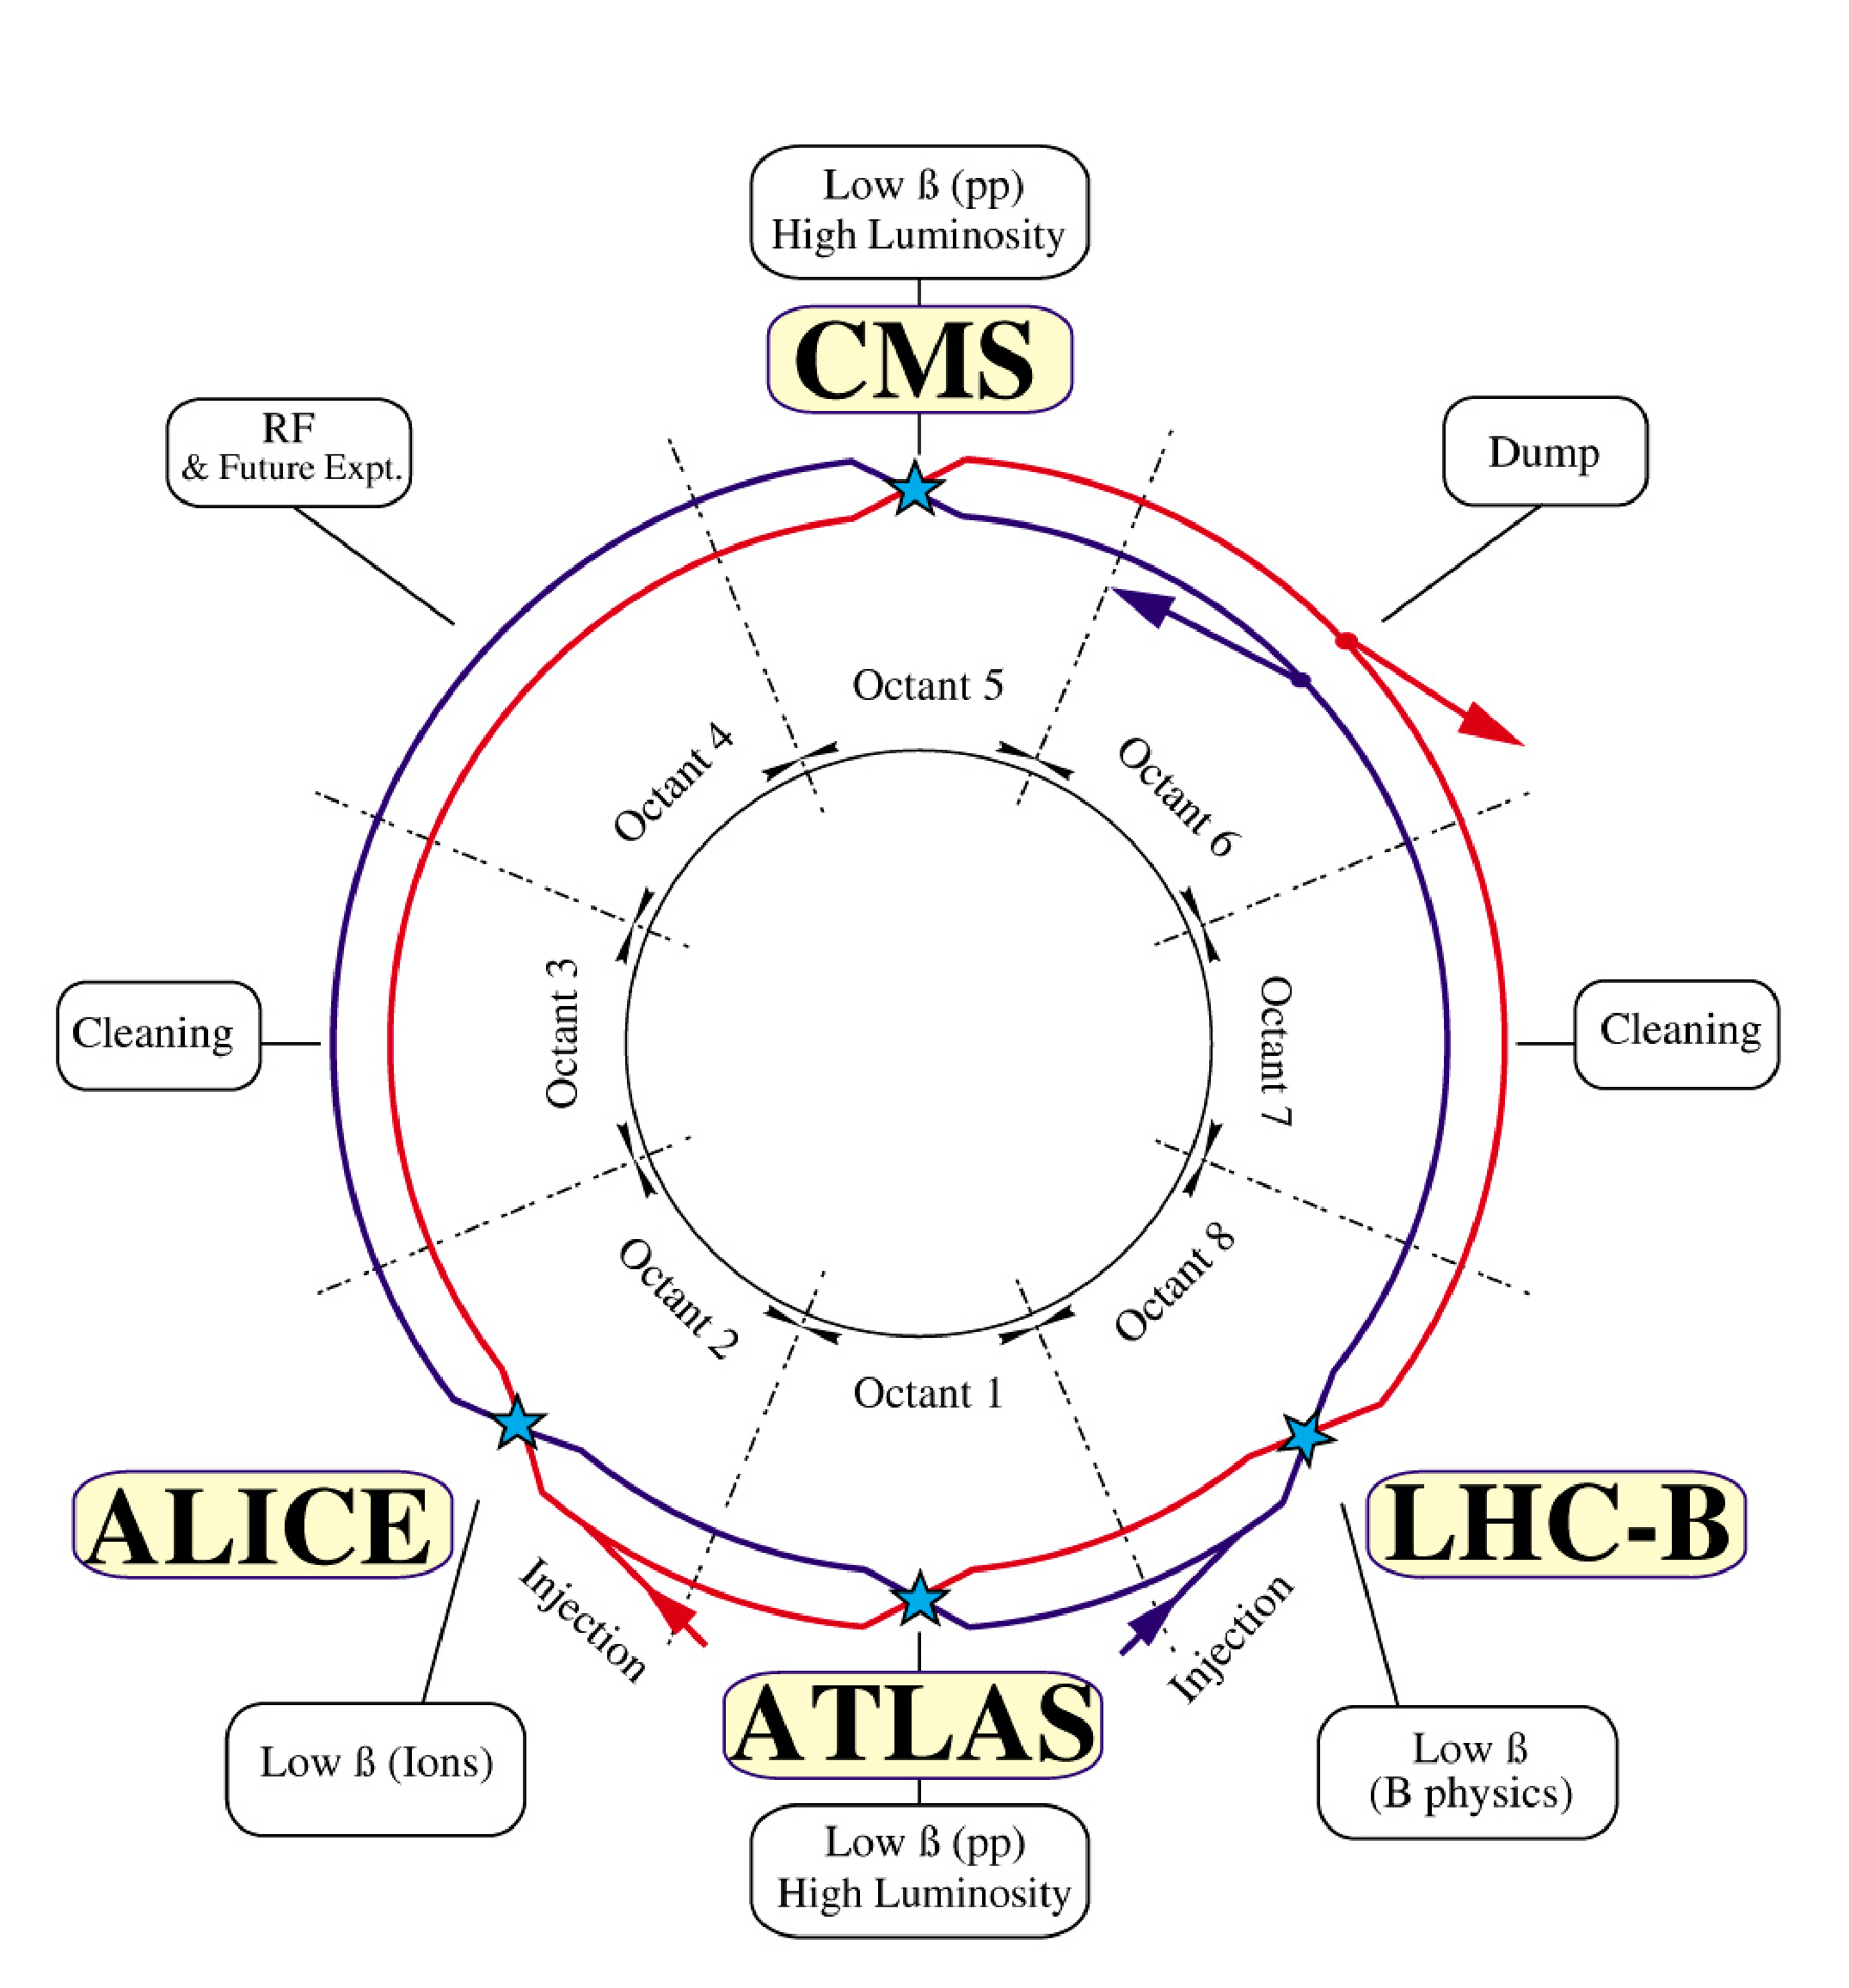
\includegraphics[width=0.60\textwidth]{plots/lhc-ring-photo.pdf}
\caption[A top down layout of the \LHC, with the position of the four main detectors labelled.]{A top down layout of the \LHC. \cite{Jean-Luc:841573}, with the position of the four main detectors labelled.}  
\label{fig:lhc-ring}
\end{figure}


Proton beams are formed inside the \acf{PS} from bunches of protons 50 \ns apart with an energy of 26 \GeV. The protons are then accelerated in the \acf{SPS} to 450 \GeV  before being injected into the \ac{lhc}. These \ac{lhc} proton beams consists of many ``bunches" i.e. approximately $1.1 \times 10^{11}$  protons localized into less than 1 \ns in the direction of motion.  Before collision the beams are ramped to 4 \TeV (2012) per beam in a process involving increasing the current passing through the dipole magnets. Once the desired \com energy is reached then the beams are allowed to collide at the interaction points. The luminosity falls regularly as the run progresses as protons are lost in collisions, and eventually the beam is dumped before repeating the process again. \\

Colliding the beams produced an instantaneous luminosity of approximately 5 $\times$ 10$^{33}$ cm$^{-2}$s$^{-1}$ during the 2012 run. The high number of protons in each bunch increases the likelihood of multiple interactions with each crossing of the counter-circulating beams. This leads to isotropic energy depositions within the detectors positioned at these interaction points, increasing the energy scale of the underlying event. This is known as pile-up and the counteracting of it's effects are important to the many measurements performed at the \ac{lhc}.

In the early phase of prolonged operation after the initial shutdown the machine operated in 2010-2011 at 3.5 \TeV per beam, \com $=$ 7 \TeV, delivering 6.13 \fb of data \cite{LHClumo}. During the 2012-2013 run period, data was collected at an increased \com $=$ 8 \TeV improving the sensitivity of searches for new physics. Over the whole run period 23.3 \fb of data was delivered of which 21.8 \fb was recorded by the \ac{CMS} detector as shown in Figure \ref{fig:lhc-lumo} \cite{LHClumo}. A total of 12 \fb of 8 \TeV certified data was collected by October 2012, and it is this data which forms the basis of the results discussed within this thesis.

\begin{figure}[!h]
\centering
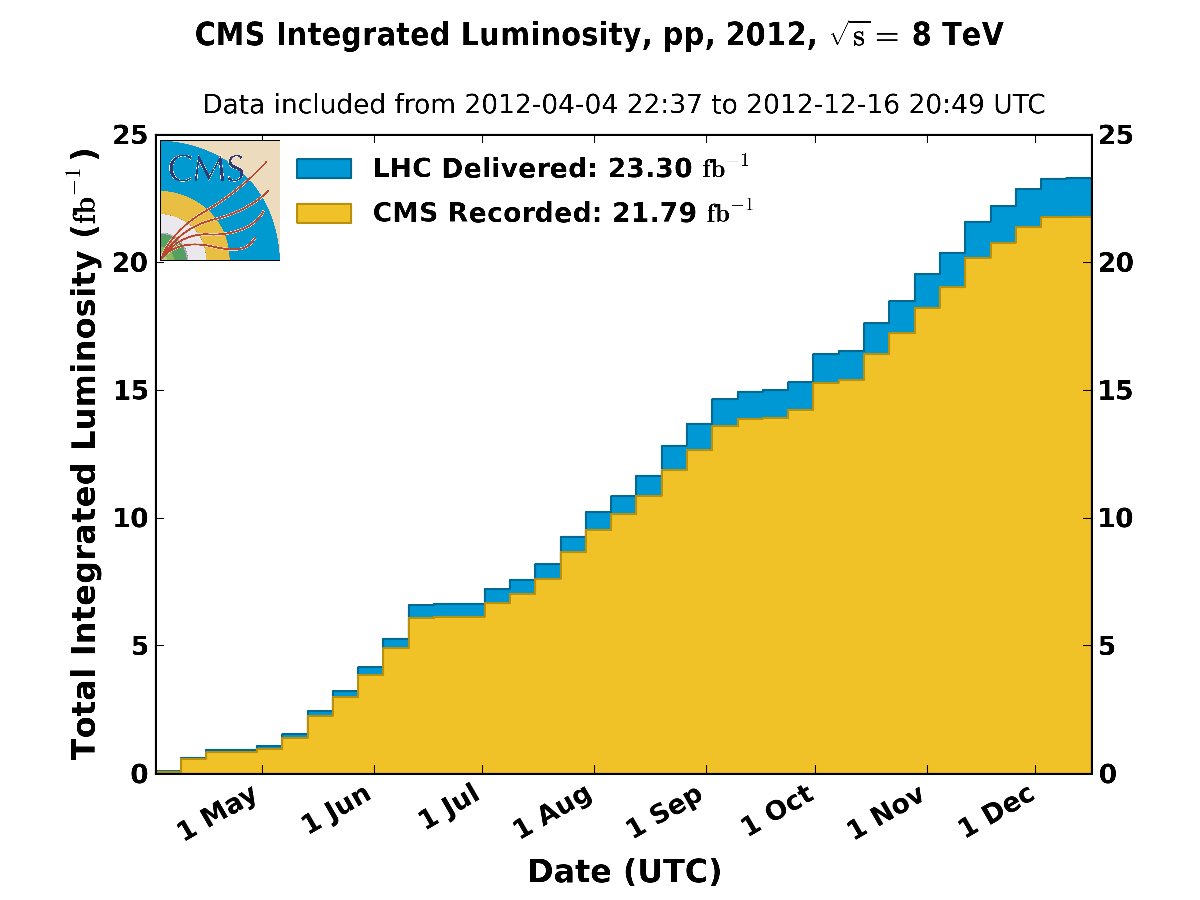
\includegraphics[width=0.60\textwidth]{plots/lhc-lumo-8tev.pdf}
\caption[The total integrated luminosity delivered to and collected by \ac{CMS} during the 2012 8 \TeV \pp runs]{The total integrated luminosity delivered to and collected by \ac{CMS} during the 2012 8 \TeV \pp runs.}  
\label{fig:lhc-lumo}
\end{figure}


\section{The CMS Detector}
\label{sec:cmsdetector}

The \acf{CMS} detector is one of two general purpose detectors at the \ac{lhc} designed to search for new physics. The detector is designed to provide efficient identification and measurement of many physics objects including photons, electrons, muons, taus, and hadronic showers over wide ranges of transverse momentum and direction. Its nearly 4$\pi$ coverage in solid angle allows for accurate measurement of global transverse momentum imbalance. These design factors give \ac{CMS} the ability to search for direct production of \ac{SUSY} particles at the \TeV scale, making the search for Supersymmetric particles one of the highest priorities among the wide range of physics programmes at \ac{CMS}. \\

\ac{CMS} uses a right-handed Cartesian coordinate system with the origin at the interaction point and the z-axis pointing along the beam axis, the x-axis points radially inwards to the centre of the collider ring, with the y-axis points vertically upward. The azimuthal angle, $\phi$ ranging between [$-\pi$,$\pi$] is defined in the x-y plane starting from the x-axis. The polar angle $\theta$ is measured from the z axis. The common convention in particle physics is to express an out going particle in terms of $\phi$ and its pseudorapidity defined as

\begin{equation}
\eta = -\log\tan\left(\frac{\theta}{2}\right).
\end{equation}

The variable $\Delta R = \sqrt{\Delta\phi^{2} + \Delta\eta^{2} } $ is commonly used to define angular distance between objects within the detector and additionally energy and momentum is typically measured in the transverse plane perpendicular to the beam line. These values are calculated from the x and y components of the object and are denoted as $\et = E\sin\theta$ and $\pt = \sqrt{p^{2}_{x}+p^{2}_{y}}$. 

\subsection{Detector subsytems}
\label{subsec:detectorsubsystems}

As the range of particles produced in \pp collisions interact in different ways with matter, \ac{CMS} is divided into subdetector systems, which perform complementary roles to identify the identity, mass and momentum of the different physics objects present in each event. These detector sub-systems contained within \ac{CMS} are wrapped in layers around a central 13 m long 4 \T super conducting solenoid as shown in Figure \ref{fig:cms-detector}. With the endcaps closed , \ac{CMS} is a cylinder of length 22 m, diameter 15 m, and mass 12.5 kilotons. A more detailed complete description of the detector can be found elsewhere \cite{cmstdr}. \\

\begin{figure}[!h]

\centering
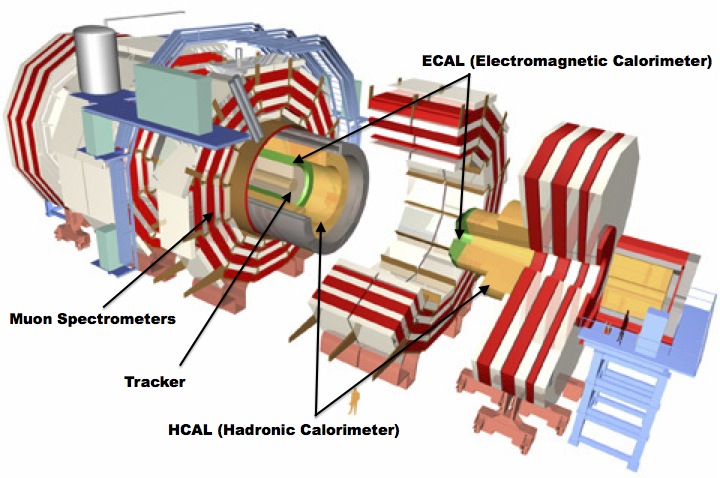
\includegraphics[width=0.65\textwidth]{plots/cms-detector.pdf}
\caption[A pictorial depiction of the \ac{CMS} detector.]{A pictorial depiction of the \ac{CMS} detector with the main detector subsystems labelled.   \cite{cms-public-detector}}  
\label{fig:cms-detector}
\end{figure}

\subsection{Tracker}
\label{subsec:tracker}

 The inner-most subdetector of the barrel is the multi-layer silicon tracker, formed of a pixel detector component encased by layers of silicon strip detectors. The pixel detector consists of three layers of silicon pixel sensors providing measurements of the momentum, position coordinates of the charged particles as they pass, and the location of primary and secondary vertices between 4cm and 10cm transverse to the beam. Outside the pixel detector, ten cylindrical layers of silicon strip detectors extend the tracking system out to a radius of 1.20m from the beam line. The tracking system provides efficient and precise determination of the charges, momenta, and impact parameters of charged particles with the geometry of the tracker extending to cover a rapidity range up to $\lvert\eta\rvert \textless$ 2.5.  \\
 
 The tracking system also plays a crucial part in the identification of jets originating from b-quarks through measurement of displaced secondary vertices, which is covered in more detail in Section (\ref{subsec:cmsobjects-btagging}). The identification of b-jets is important in many searches for natural \ac{SUSY} models and forms an important part of the inclusive search strategy described within Section (\ref{subsec:searchstrategy}).
 
\subsection{Electromagnetic calorimeter}
\label{subsec:ecal}

 Immediately outside of the tracker, but still within the magnet core, sits the \acf{ECAL}. Covering a pseudorapididity up to $\lvert\eta\rvert < 3$ and compromising of over 75,000 PbWO$_{4}$ (lead tungstate) crystals that scintillate as particles deposit energy, the \ac{ECAL} provides high resolution measurements of the electromagnetic showers from photons, electrons in the detector. \\ 
 
 Lead tungstate is used because of its short radiation length ($X_{0} \sim 0.9$cm) and small Molier\'{e} radius ($\sim 2.1$cm) leading to high granularity and resolution. It's fast scintillation time ($\sim 25$ns) reduces the effects of pile-up due to energy from previous collisions still being read out, and its radiation hardness gives it longevity. The crystals are arranged in modules which surround the beam line in a non-projective geometry,  angled at 3$^{\circ}$ with respect to the interaction point to minimise the risk of particles escaping down the cracks between the crystals.\\
 
 The  \ac{ECAL} is primarily composed of two sections, the \acf{EB} which extends in pseudo-rapidity to $\lvert\eta\rvert < 1.479$ with a crystal front cross section of 22$\times$22 mm and a length of 230 mm corresponding to 25.8 radiation lengths, and the \acf{EE} covering a rapidity range of $1.479 < \lvert\eta\rvert < 3.0 $, which consists of two identical detectors
on either side of the \ac{EB}.  A lead-silicon sampling `pre-shower' detector \acf{ES} is placed before the endcaps to aid in the identification of neutral pions. Their arrangement are shown in Figure \ref{fig:cms-ecal}. \\

 
 \begin{figure}[!h]

\centering
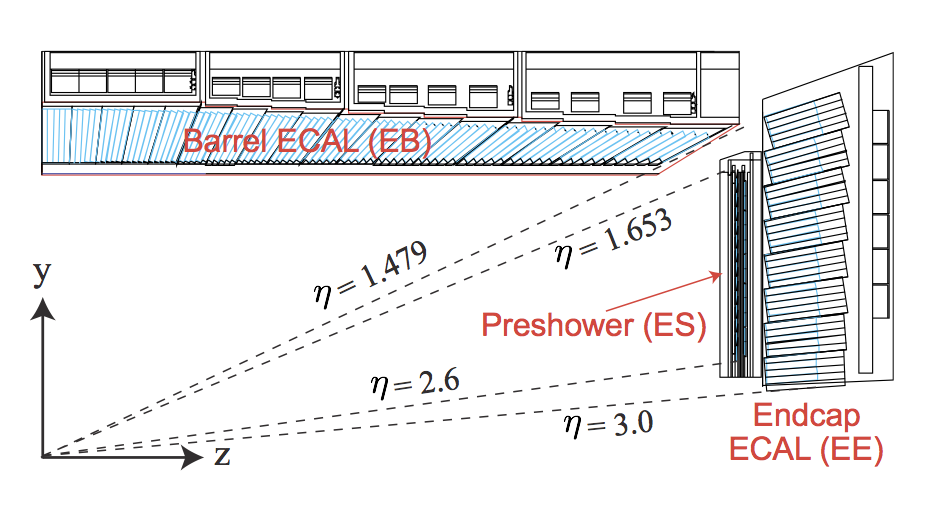
\includegraphics[width=0.85\textwidth]{plots/cms-ecal.pdf}
\caption[Illustration of the \ac{CMS} \ac{ECAL}. ]{Illustration of the \ac{CMS} \ac{ECAL} showing the arrangement of the lead tungstate crystals in the \ac{EB} and \ac{EE}. The \ac{ES} is also shown and is located infront of the \ac{EE} \cite{CMS_ECAL_TDR}.}  
\label{fig:cms-ecal}
\end{figure}


Scintillation photons from the lead tungstate crystals are instrumented with \acf{APD} and \acf{VPT} located in the \ac{EB} and \ac{EE} respectively, converting the scintillating light into an electric signal which is consequently used to determine the amount of energy deposited within the crystal . These instruments are chosen for their resistance under operation to the strong magnetic field of \ac{CMS}. The scintillation of the \ac{ECAL} crystals as well as the response of the \ac{APD}s varies as a function of temperature and so cooling systems continually maintain an overall constant \ac{ECAL} temperature $\pm 0.05 ^{\circ}C$.
 

\subsection{Hadronic calorimeter}
\label{subsec:hcal} 

Beyond the \ac{ECAL} lies the \acf{HCAL} which is responsible for the accurate measurement of hadronic showers, crucial for analyses involving jets or missing energy signatures. The \ac{HCAL} is a sampling calorimeter which consists of alternating layers of brass absorber and plastic scintillator, except in the hadron forward ($3.0 < \lvert\eta\rvert < 5.0 $) region in which steel absorbers and quartz fibre scintillators are used because of their increased radiation tolerance. Hadron showers are initiated in the absorber layers inducing scintillation in the plastic scintillator tiles.  These scintillation photons are converted by wavelength shifting fibres for read-out by hybrid photodiodes. \\

The \ac{HCAL}'s size is constrained to a compact size by the presence of the solenoid, requiring the placement of an additional outer calorimeter on the outside of the solenoid to increase the sampling depth of the \ac{HCAL}. A schematic of the \ac{HCAL} can be seen in Figure \ref{fig:cms-hcal}.\\
 
 \begin{figure}[!h]

\centering
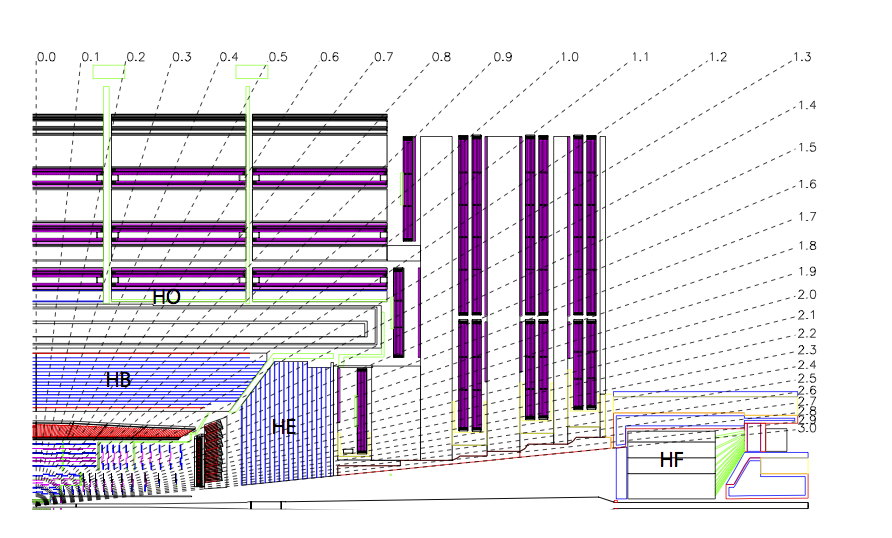
\includegraphics[width=0.85\textwidth]{plots/cms-hcal.pdf}
\caption[Schematic of the \ac{CMS} \acf{HCAL}.]{ Schematic of the hadron calorimeters in the r-z plane, showing the locations of the \ac{HCAL} components and the \ac{HF}. \cite{cmstdr}.}  
\label{fig:cms-hcal}
\end{figure}
 
The \ac{HCAL} covers the range $\lvert\eta\rvert < 5$ and consists of four subdetectors: the \ac{HB}  $\lvert\eta\rvert < 1.3$, the \acf{HO}, the \acf{HE} $1.3 < \lvert\eta\rvert < 3.0 $ and the \acf{HF}.  The \ac{HB}, contained between the outer edge of the \ac{ECAL} and the inner edge of the solenoid is formed of 36 azimuthal wedges which are split between two half-barrel segments. Each wedge is segmented into four azimuthal angle ($\phi$) sectors, and each half-barrel is further segmented into 16 $\eta$ towers. The electronic readout chain, channels the light from the active scintillator layers from one $\phi$-segment and all $\eta$-towers of a half-barrel to a \acf{HPD}.

The relatively short number of interaction lengths ($\lambda_{l}$, the distance a hadron will travel through the absorber material before it has lost $\frac{1}{e}$ of its energy) within the \ac{HB}, the lowest being $\lambda_{l}$ = 5.82 for $\lvert\eta\rvert = 0$, facilitates the need for the `tail catching' \ac{HO} to increase the sampling depth in the central barrel rapidity region $\lvert\eta\rvert < 1.3$ to 11 interaction lengths . Significant fractions of the hadrons energy will be deposited in the \ac{ECAL} as it passed through the detector. Therefore measurements of hadron energies in the central regions $\lvert\eta\rvert < 3.0$ use both the \ac{ECAL} and \ac{HCAL} to reconstruct the true energy from showering hadrons. 

\subsection{Muon systems}
\label{subsec:muonsystems} 
 
Muons being too massive to radiate away energy via Bremsstrahlung, interact little in the calorimeters and mostly pass through the detector until they reach the system of muon detectors which forms the outer most part of the \ac{CMS} detector.  

Outside of the superconducting solenoid are four muon detection layers interleaved with the iron return yokes which measure the muons energy via ionisation of gas within detector elements. Three types of gaseous chamber are used. The \acf{DT}, \acf{CSC}, and \acf{RPC} systems provide efficient detection of muons with pseudo-rapidity $\lvert\eta\rvert < 2.4 $. The best reconstruction performance is obtained when the muon chamber is combined with the inner tracking information to determine muon trajectories and their momenta \cite{CMS_MUON_TDR}.  \\ 

\section{Event Reconstruction and Object Definition}
\label{sec:cmsobjects}

The goal of event reconstruction is to take the raw information recorded by the detector and to compute from it higher-level quantities which can be used at an analysis level. These typically correspond to an individual particle's energy and momenta, or groups of particles which shower in a narrow cone and the overall global energy and momentum balance of the event. The reconstruction of these objects are described in great detail in \cite{CMS_TDR_PHYS_vol1}, however covered below are brief descriptions of those which are most relevant to the analysis detailed in Chapter \ref{chap:SUSYsearches}.

\subsection{Jets}
\label{subsec:cmsobjects-jets}

Quarks and gluons are produced copiously at the LHC in the hard scattering of partons. As these quarks and gluons fragment, they hadronise and decay into a group of strongly interactive particles and their decay products. These streams of particles travel in the same direction, as they have been "boosted" by the momentum of the primary hadron. These collections of decay products are reconstructed and identified together as a ``jet''.

At \ac{CMS} jets are reconstructed from energy deposits in the detector using the anti-kt algorithm \cite{antiktalgo} with size parameter $\Delta R = 0.5$. The anti-kt jet algorithm clusters jets by defining a distance between hard (high $\pt$) and soft (low $\pt$) particles such that soft particles are preferentially clustered with hard particles before being clustered between themselves. This produces jets which are robust to soft particle radiation from the pile-up conditions produced by the \ac{lhc}. \\

There are two main type of jet reconstruction used at \ac{CMS}, Calorimeter (\Calo) and Particle Flow (\PF) jets \cite{CMS-PAS-JME-10-003}. Calorimeter jets are reconstructed using both the \ac{ECAL} and \ac{HCAL} cells, combined into calorimeter towers . These calorimeter towers consist of geometrically matched \ac{HCAL} cells and \ac{ECAL} crystals. Electronics noise is suppressed by applying a threshold to the calorimeter cells, with pile-up effects reduced by a requirement placed on the tower energy  \cite{Janssen:1322145}. Calorimter jets are the jets used within the analyses described in this thesis.  

\PF jets are formed from combining information from all of the \ac{CMS} subdetectors systems to  determine which final state particles are present in the event. Generally, any particle is expected to produce some combination
of a track in the silicon tracker, a deposit in the calorimeters, or a track in the muon system. The \PF jet momentum and spatial resolutions are greatly improved with respect to calorimeter jets, as the use of the tracking detectors and of the high granularity of \ac{ECAL} allows resolution and measurement of charged hadrons and photons inside a jet,  which together constitute $\sim$ 85$\%$ of the jet energy \cite{1748-0221-6-11-P11002}.

The jets reconstructed by the clustering algorithm in \ac{CMS} typically have an energy that differs to the `true' energy measured by a perfect detector. This stems from the non-linear and nonuniform response of the calorimeters as well as other residual effects including pile-up and underlying events, and therefore additional corrections are applied to recover a uniform relative response as a function of pseudo-rapidity. These are applied as separate sub corrections \cite{1742-6596-404-1-012014}. 

\begin{itemize}

\item A PU correction is first applied to the jet. It subtracts the average extra energy deposited in the jet that comes from other vertices present in the event and is therefore not part of the hard jet itself.
\item $\pt$ and $\eta$ dependant corrections derived from Monte Carlo simulations are used to account for the non-uniform response of the detector.\item $\pt$ and $\eta$ residual corrections are applied to data only to correct for difference between data and Monte Carlo. The residual is derived from QCD dijet samples and the $\pt$ residual from $\gamma + $ jet and $Z + $ jets samples in data.

\end{itemize}

\subsection{B-tagging}
\label{subsec:cmsobjects-btagging}

The decays of b quarks are suppressed by small \CKM matrix elements. As a result, the lifetimes of b-flavoured hadrons, produced in the fragmentation of b quarks, are relatively long; $\mathcal{O}$ 1ps. The identification of jets originating from b quarks is very important for searches for new physics and for measurements of standard model processes.  \\

Many different algorithms developed by \ac{CMS} select b-quark jets based on variables such as the impact parameters of the charged-particle tracks, the properties of reconstructed decay vertices, and the presence or absence of a lepton, or combinations thereof \cite{CMS-PAS-BTV-09-001}. One of the most efficient of which is the \acf{CSV} which operates based on secondary vertex and track-based lifetime information, benchmarked in `Loose', `Medium' and `Tight' working points, of which the medium point is the tagger used within the \alphat search detailed in Section (\ref{sec:alphatintroduction}).

Using the \ac{CSV} tagger, a likelihood-based discriminator distinguishes between jets from b-quarks, and those from charm or light quarks and gluons, which is shown in Figure \ref{fig:btagdescrims}. The minimum thresholds on the discriminator for each working point correspond to the misidenti�cation probability for light-parton jets of 10$\%$, 1$\%$, and 0.1$\%$, respectively, in jets with an average $\pt$ of about 80 \GeV. 

\begin{figure}[ht]
\centering
\begin{minipage}[b]{0.70 \linewidth}
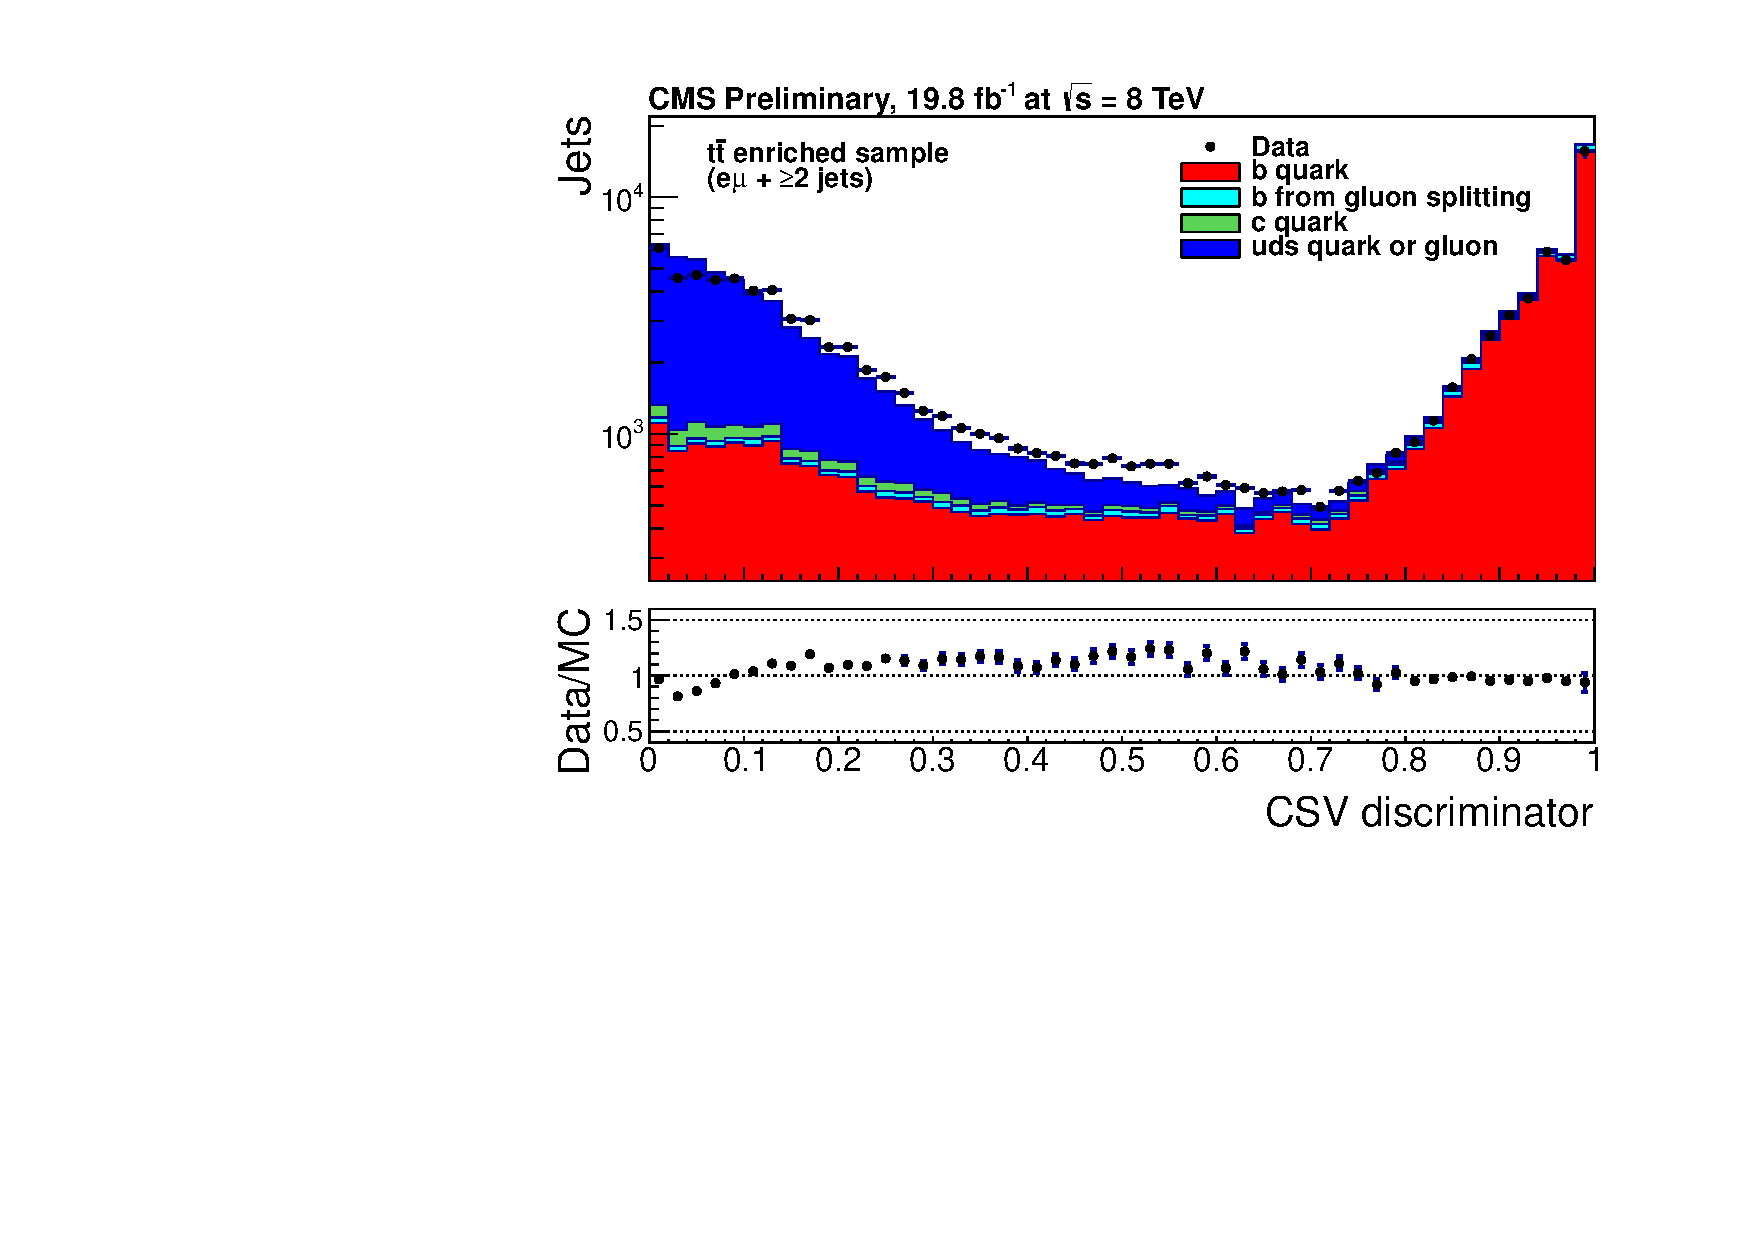
\includegraphics[width = 1.0\linewidth]{plots/btag-ttbardiscrim.pdf}
\end{minipage}
\quad
\begin{minipage}[b]{0.70\linewidth}
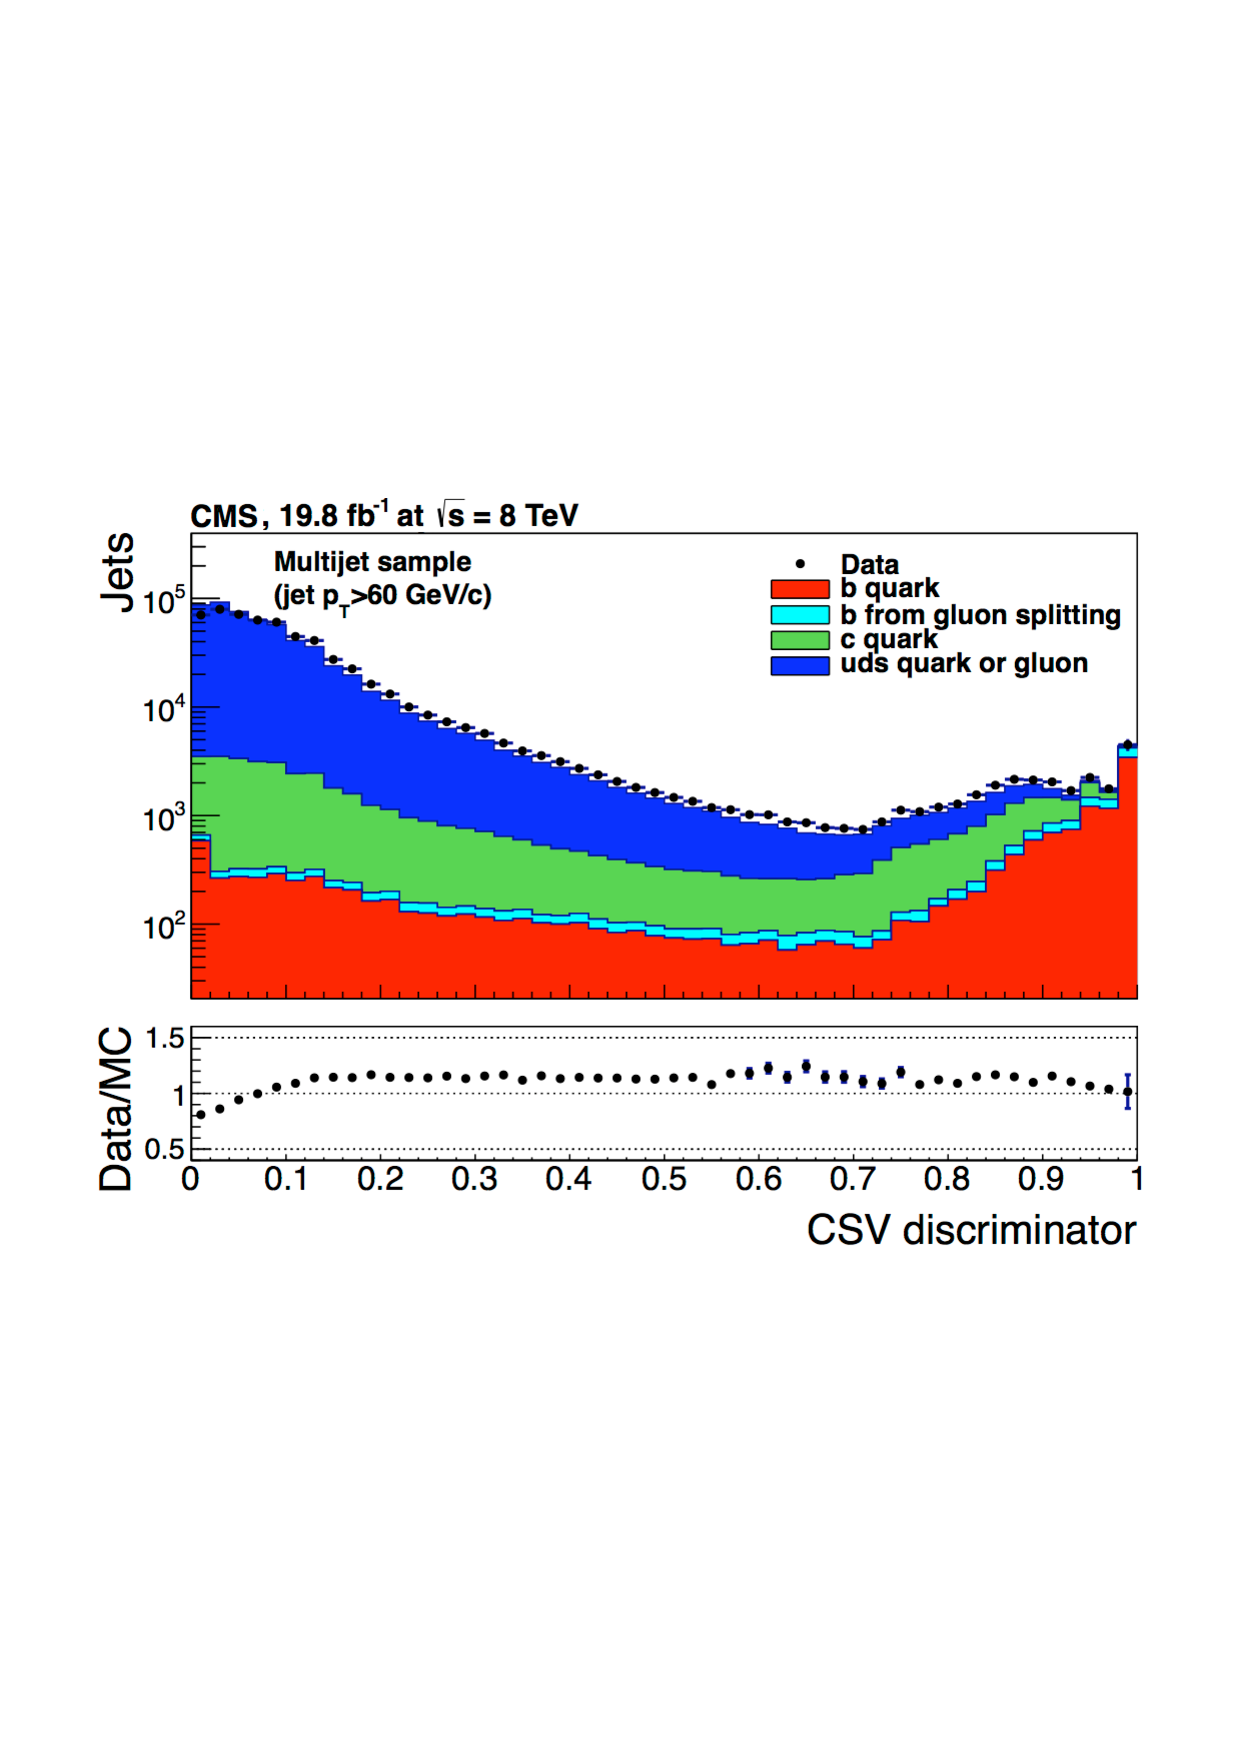
\includegraphics[width = 1.0\linewidth]{plots/btag-multijetdiscrim.pdf}
\end{minipage}
\caption[ \ac{CSV} algorithm discriminator values in enriched ttbar and inclusive multi jet samples]{\ac{CSV}algorithm discriminator values in enriched ttbar (top) and inclusive multi jet samples (bottom) for b,c and light flavoured jets \cite{btag8tev}. Working points are determined from the misidentification probability for light-parton jets to be tagged as a b-jet and are given as 0.244, 0.679 and 0.898 for L,M and T working points respectively. }
\label{fig:btagdescrims}
\end{figure}

The b-tagging performance is evaluated to measure the b-jet tagging efficiency \effb, and the misidentification probability of charm \effc and light-parton jets \effs . The tagging efficiencies for each of these three jet flavours are compared between data and MC simulation, from which a series of $\pt$ and $\lvert\eta\rvert$ binned jet corrections are determined,

\begin{equation}
SF_{b,c,s} = \frac{\epsilon^{data}_{b,c,s}}{\epsilon^{MC}_{b,c,s}} .
\end{equation}

These are collectively named `Btag Scale Factors' and allow MC simulation to accurately reflect the running conditions and performance of the tagging algorithm in data. Understanding of the b-tagging efficiency is essential in order to minimise systematic uncertainties in physics analyses that employ b-tagging. \\
 
The b-tagging efficiency is measured in data using several methods applied to multi jet events, primarily based on a sample of jets enriched in heavy flavour content. One method requires the collection of events with a soft muon within a cone $\Delta R < 0.4$ around the jet axis. Because the semileptonic branching fraction of b hadrons is significantly larger than that for other hadrons, these jets are more likely to arise from b quarks than from another flavour, with the resultant momentum component of the muon transverse to the jet axis larger for muons from b-hadron decays than from light or charm jets.  Additionally the performance of the tagger can also be benchmarked in \ttbar events where in the \ac{SM}, the top quark is expected to decay to a W boson and a b quark about 99.8$\%$ of the time \cite{pdg2012}. Further selection criteria is applied to these events to further enrich the b quark content of these events. The methods to identify b-jets in data are discussed in great detail at \cite{btag7tev}. The jet flavours are determined in simulation using truth level information and are compared to data to determine the correction scale factors ($SF_{b}$), which are displayed for the \ac{CSVM} tagger in Figure \ref{fig:btagscalefactors}. 

\begin{figure}[ht]
\centering
\begin{minipage}[b]{0.31 \linewidth}
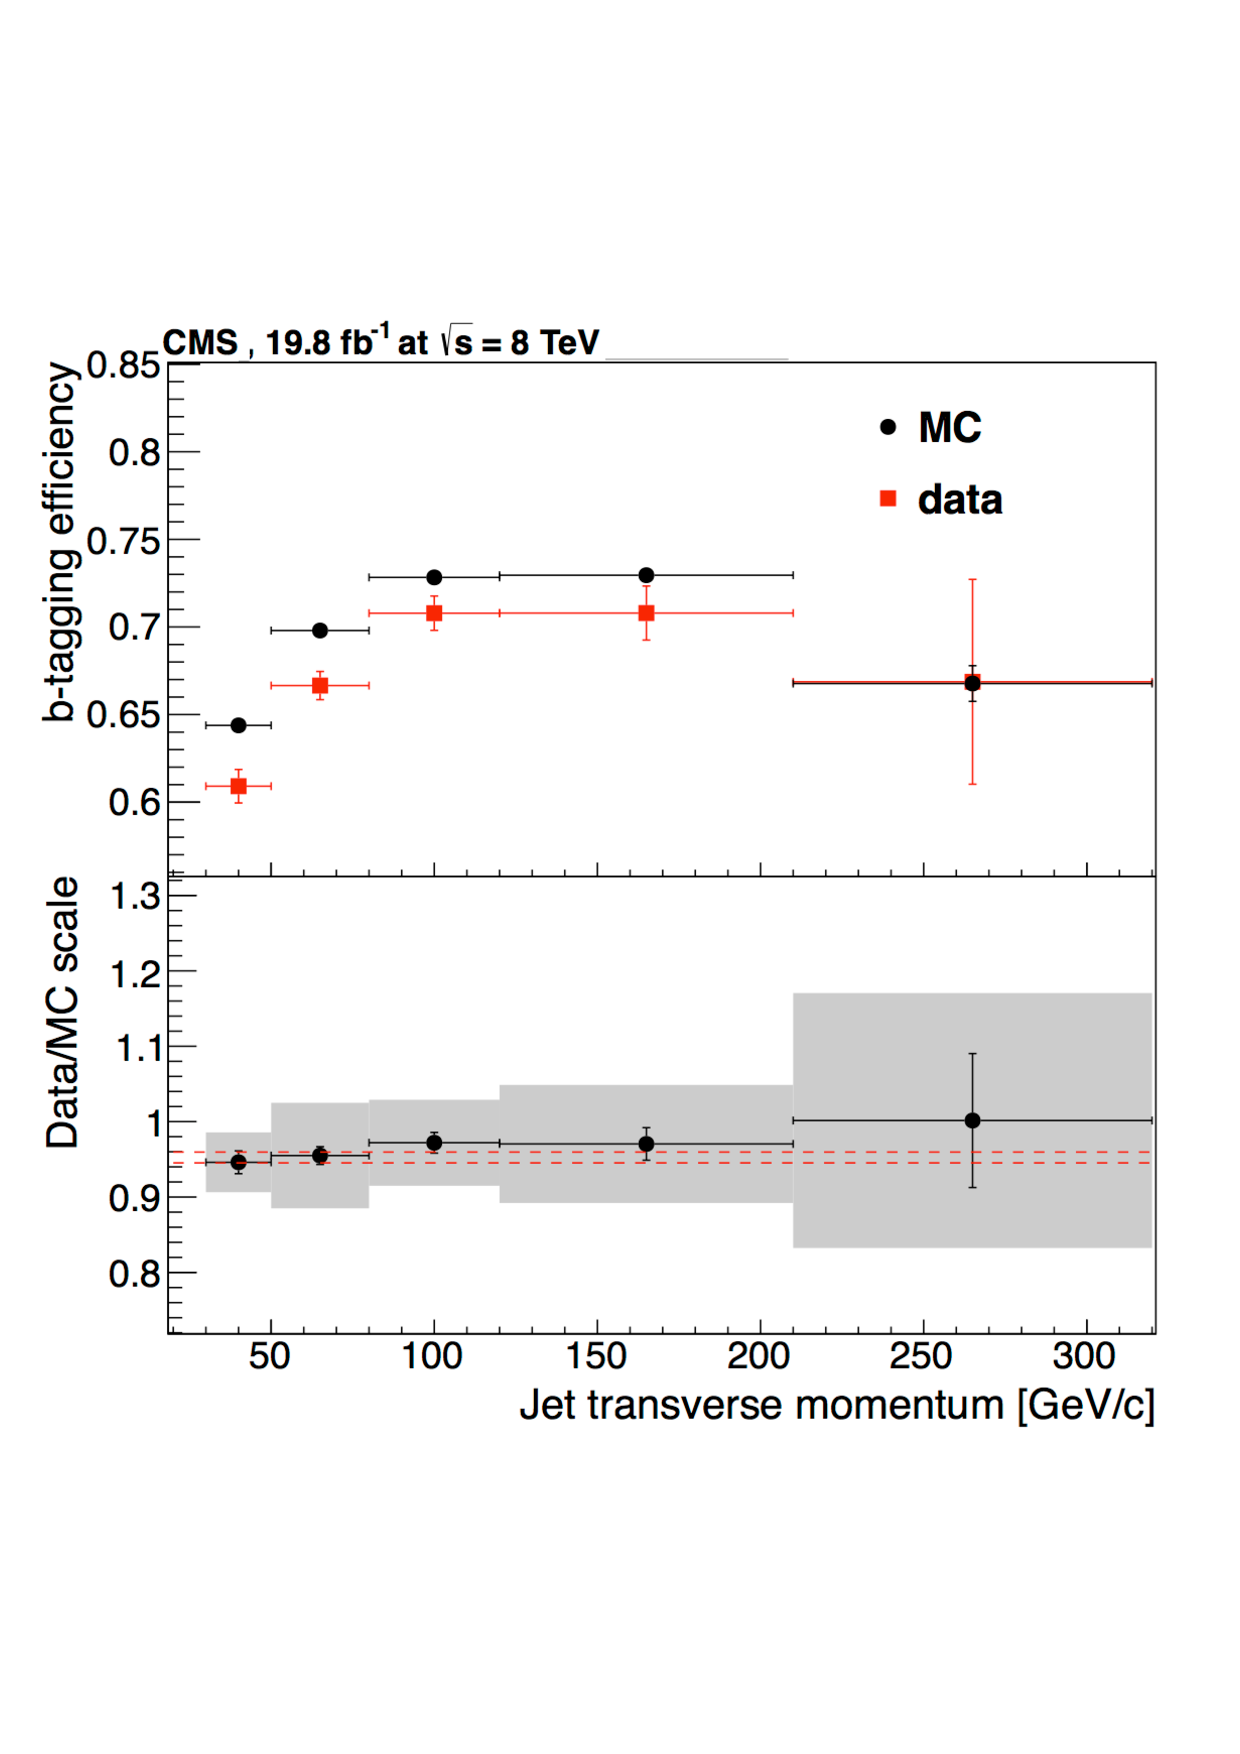
\includegraphics[width = 1.0\linewidth]{plots/btag-csvm_pt_sf.pdf}
\end{minipage}
\quad
\begin{minipage}[b]{0.31\linewidth}
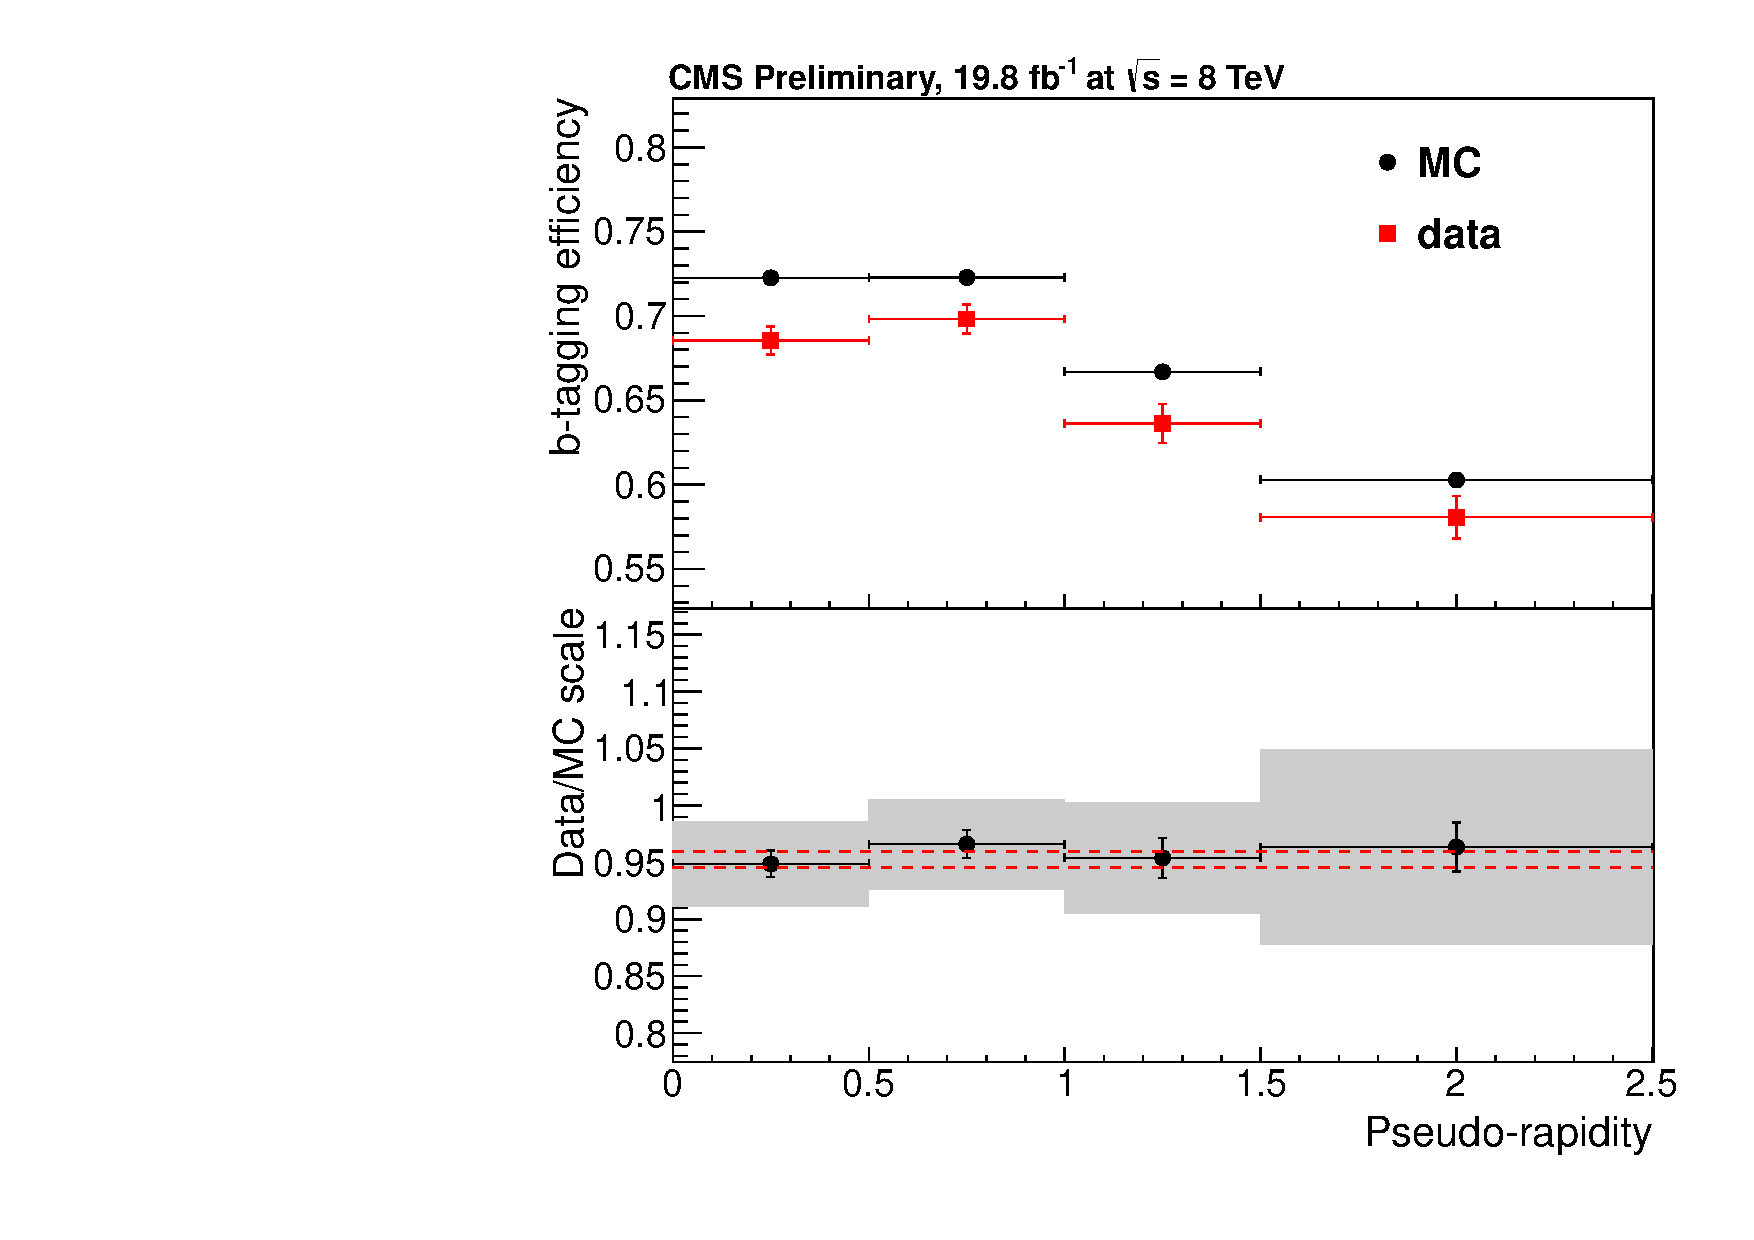
\includegraphics[width = 1.0\linewidth]{plots/btag-csvm_eta_sf.pdf}
\end{minipage}
\quad
\begin{minipage}[b]{0.31\linewidth}
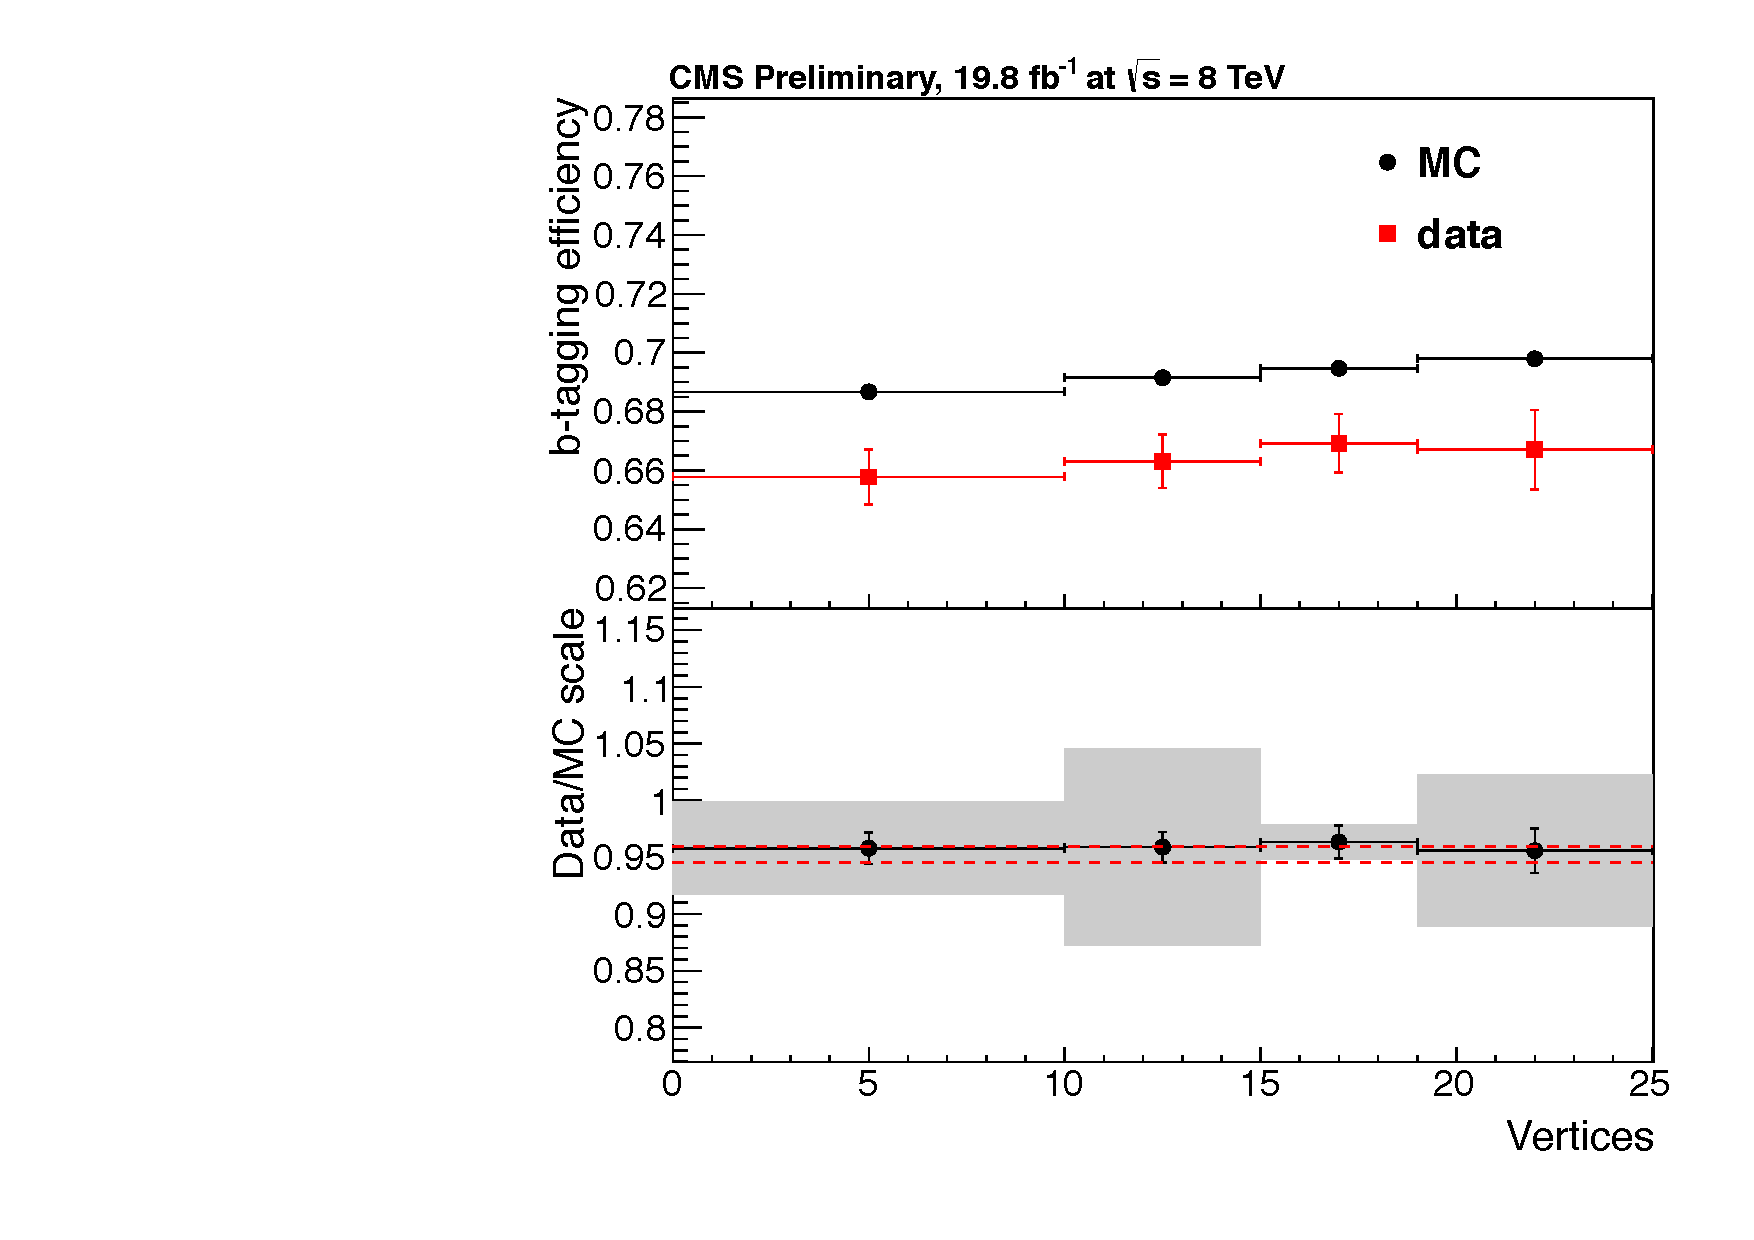
\includegraphics[width = 1.0\linewidth]{plots/btag-csvm_vert_sf.pdf}
\end{minipage}
\caption[Data/MC b-tag scale factors derived using the \ac{CSVM} tagger.]{Measured in \ttbar $\rightarrow$ di-lepton events using the \ac{CSVM} tagger: (upper panels) b-tagging efficiencies and (lower panels) data/MC scale factor $SF_{b}$ as a function of (left) jet $\pt$, (middle) jet $\lvert\eta\rvert$ and (right) number of primary vertices. In the lower panels, the grey filled areas represent the total statistical and systematic uncertainties, whereas the dotted lines are the average $SF_{b}$ values within statistical uncertainties.}
\label{fig:btagscalefactors}
\end{figure}

The measurement of the misidenti�cation probability for light-parton jets relies on the inversion of tagging algorithms, selecting non-b jets using the same variables and techniques used in benchmarking the b-tagging efficiency. The scale factors ($SF_{s}$) to be applied to MC are shown in Figure \ref{fig:mistagscalefactors} for the \ac{CSVM} tagger.

\begin{figure}[ht]
\centering
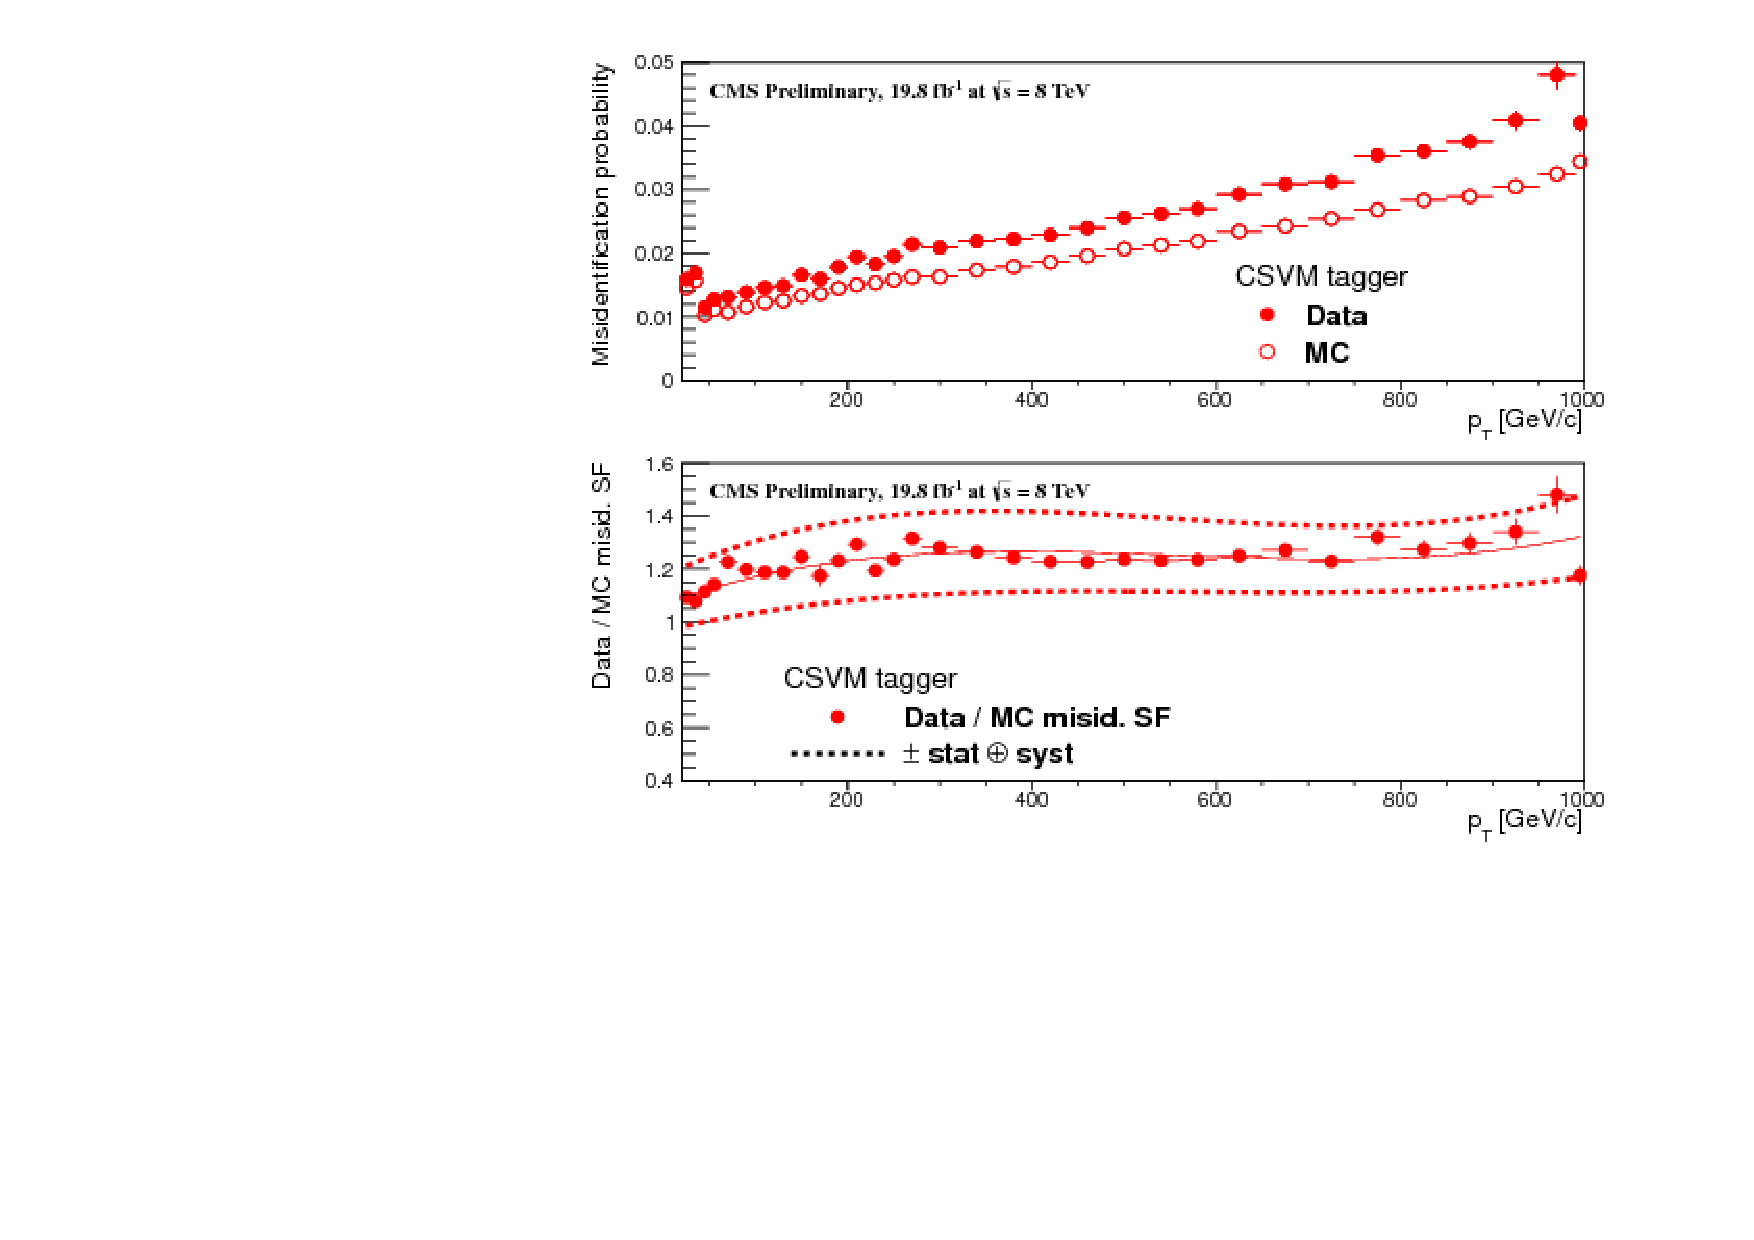
\includegraphics[width=0.70\linewidth]{plots/btag-csvmsf_v2.pdf}
\caption[Data/MC mis-tag scale factors derived using the \ac{CSVM} tagger.]{For the \ac{CSVM} tagging criterion: (top) misidenti�cation probability in data (filled circles) and simulation (open circles); (bottom) scale factor for the misidenti�cation probability. The last $\pt$ bin in each plot includes all jets with $\pt > 1000$ \GeV. The solid curve is the result of a polynomial fit to the data points. The dashed curves represent the overall statistical and systematic uncertainties on the measurements.}  

\label{fig:mistagscalefactors}
\end{figure}


\section{Triggering System}

\label{sec:triggersystem}

With bunch crossings separated by just 25 ns, the rate at which data from all collisions would have to be written out and processed would be unfeasible. A two-tiered triggering system is applied at \ac{CMS} in order to cope with the high collision rate of protons. The \ac{CMS} trigger is designed to use limited information from each event to determine whether to record the event, reducing the rate of data taking to manageable levels whilst ensuring a high efficiency of interesting physics object events are selected.

The \ac{L1} is a pipelined, dead-timeless system based on custom-built electronics \cite{Dasu:2000ge}, and is a combination of several sub systems which is shown pictorially in Figure \ref{fig:l1triggersystem}. The \L1 system is covered in more detail within the following section along with a description of the service work undertaken by the author to benchmark the performance of the \L1 calorimeter trigger during the 2012 8 \TeV run period.


\begin{figure}[ht]
\centering
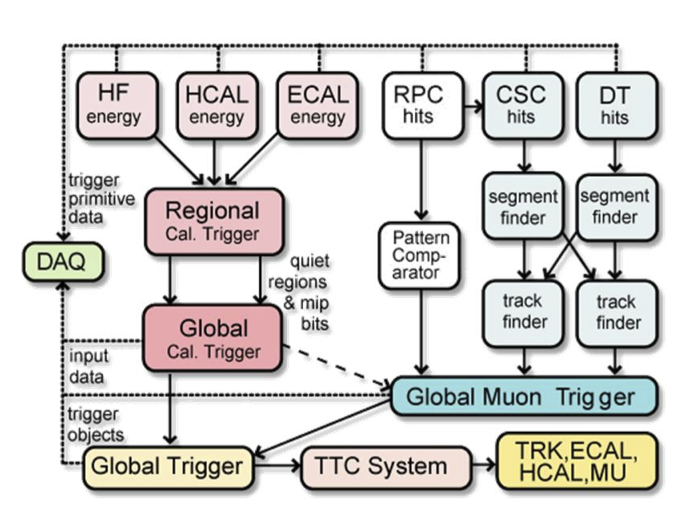
\includegraphics[width=0.80\textwidth]{plots/l1triggersystem.pdf}
\caption[The \ac{CMS} \ac{L1} Trigger system.]{The \ac{CMS} \ac{L1} Trigger system.}  
\label{fig:l1triggersystem}
\end{figure}



The \acf{HLT} is a large farm of commercial computers \cite{Sphicas:2002gg}. The \ac{HLT} processes events with software reconstruction algorithms that are more detailed, giving performance more similar to the reconstruction used offline. The \ac{HLT} reduces the event rate written to disk by a factor of $\sim$ 500 ($\sim$200Hz). The recorded events are transferred from \ac{CMS} to the \ac{CERN} computing centre, where event reconstruction is performed, and then distributed to \ac{CMS} computing sites around the globe for storage and analysis.

\subsection{The level-1 trigger}
\label{subsec:l1trigger}

The \L1 trigger reduces the rate of events collected from 40 MHz to $\sim$100 kHz using information from the calorimeters and muon chambers, but not the tracker. A tree system of triggers is used to decide wether to pass on an event to the \ac{HLT} for further reconstruction. Firstly the calorimeter and muon event information is kept separate, with local reconstruction of objects ($\mu$,e,$\gamma$,jets) performed by the \acf{RCT} and \acf{RMT} respectively. The \ac{RCT} generates up to 72 isolated and non-isolated electromagnetic objects. These are sorted by rank, which is equivalent to transverse energy $\et$, with the four highest ranked electromagnetic objects being passed via the  \acf{GCT} and \acf{GMT} to the \acf{GT}. 

In the \L1 \ac{GCT}, coarse measurements of the energy deposited in the electromagnetic and hadronic calorimeters are combined and by using sophisticated algorithms the following physics objects are formed:

\begin{itemize}
	\item isolated and non-isolated electromagnetic objects (e and $\gamma$);
	\item hadronic jets in the central and forward sections of the hadronic calorimeters;
	\item hadronically decaying tau leptons;
	\item total transverse energy ($\et$), the scalar sum of the energy measured at L1,  and missing transverse energy ($\met$), defined as the vector sum of the energy of L1 objects; 
	\item total transverse jet energy ($\theht$), the scalar sum of the energy of all L1 jet objects, and missing transverse jet energy ($\mht$), defined as  the vector sum of the energy of L1 jets, are calculated from uncorrected \L1 jets. 
\end{itemize}

In addition quantities suitable for triggering minimum bias events, forward physics and beam background events are calculated. Additionally relevant muon isolation information is also passed on to the \ac{GMT} for decisions involving the muon triggers where it is combined with information from across the three muon sub-systems. The resultant final accept/reject decision at \ac{L1} is then performed by the \ac{GT} based on the objects received from the \ac{GCT} and \ac{GMT} ($e/\gamma$, $\mu$, jets, $\et$, $\met$, $\theht$).

The \L1 trigger is therefore of upmost importance to the functioning of the detector. Without a high-performing trigger and a good understanding of it's performance, there would be no data to analyse. Observations of how the \L1 trigger performance is affected by changing \ac{lhc} running conditions over the 2012 run period and also the introduction of a jet seed threshold to the \L1 jet trigger algorithm is presented in the following Sections (\ref{subsec:l1jettrigger} - \ref{subsec:l1summary}).

\subsection{The \L1 trigger jet algorithm}
\label{subsec:l1jettrigger}

The \L1 jet trigger uses the transverse energy sums computed in the calorimeter (both hadronic and electromagnetic) trigger regions. Each region consists of $4 \times 4 $  trigger tower windows, spanning a region of $\Delta \eta \times \Delta \phi = 0.087 \times 0.087$ in pseudorapidity-azimuth. The jet trigger uses a $3 \times 3$ calorimeter region (112 trigger towers) sliding window technique which spans the full $(\eta, \phi)$ coverage of the \ac{CMS} calorimeter as shown in Figure \ref{fig:l1jetalgo}. 

In forming a \L1 jet is it required that the central region to be higher than the eight neighbouring regions $ E_{T central} > E_{T surround}$. Additionally a minimum threshold of 5 \GeV on $E_{T central}$ was introduced during the 2012 run period to suppress noise from pile-up, the effects of which are shown in Section (\ref{subsec:l1jetseedpu}).

The \L1 jets are characterised by the $\et$, summed over the $3 \times 3$ calorimeter regions, which corresponds to $12 \times 12$ trigger towers in barrel and endcap or $3 \times 3$ larger \ac{HF} towers in the \ac{HF}. The $\phi$ size of the jet window is the same everywhere, whilst the $\eta$ binning gets somewhat larger at high $\eta$ due to calorimeter and trigger tower segmentation. The jets are labelled by $(\eta, \phi)$ indexes of the central calorimeter region.                                                                                                                                                  

Jets with $|\eta|>3.0$ are classified as forward jets, whereas those with $|\eta|<3.0$ are classified as central. The four highest energy central, forward and $\tau$ jets in the calorimeter are passed through \acf{LUT}'s, which apply a programmable $\eta-$dependent jet energy scale correction. These are then used to make \L1 trigger decisions.

\begin{figure}[ht!]
\centering
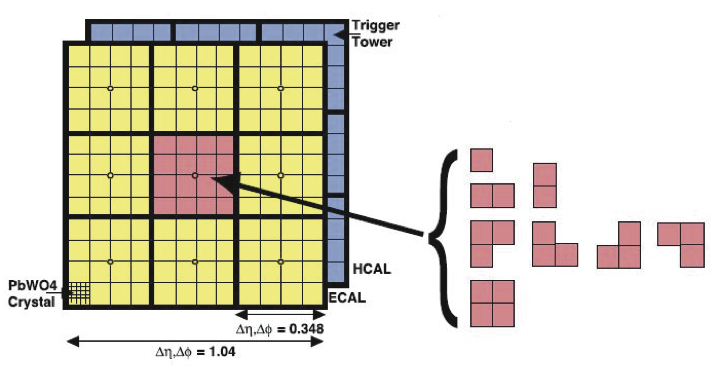
\includegraphics{plots/L1JetAlgorithm.pdf}
\caption[Illustration of the Level-1 jet finding algorithm.]{Illustration of the Level-1 jet finding algorithm.}  
\label{fig:l1jetalgo}
\end{figure}  

The performance of the \L1 jets is evaluated with respect to offline jets, which are taken from the standard \Calo jet and the \PF jet reconstruction algorithms of \ac{CMS}. Jets are corrected for pile-up and detector effects as described in \ref{subsec:cmsobjects-jets}. A moderate level of noise rejection is applied to the offline jets by selecting jets passing the ``loose� identification criteria for both \Calo and \PF. These criteria are summarised in Appendix (\ref{app:noise}). 


\subsection{Measuring \L1 jet trigger efficiencies}
\label{subsec:l1jettrigeff}

The \L1 jet efficiency is defined as the fraction of leading offline jets which were matched with a L1 tau or central jet above a certain trigger threshold, divided by all the leading offline jets in the event. This quantity is then plotted as a function of the offline jet $\et$, $\eta$ and $\phi$. 

The efficiency is determined by matching the \L1 and reconstructed offline jets spatially in $\eta - \phi$ space.  This is done by calculating the minimum separation in $\Delta R$ between the highest offline reconstructed jet in $\et$ ($\et>10$~GeV,$\lvert\eta\rvert<3$) and any \L1 jet. A jet will be matched if this value is found to be $< 0.5$. Should more than one jet satisfy this, the jet closest in $\Delta R$ is taken as the matched jet. The matching efficiency is close to 100$\%$, above 30(45) GeV for run 2012B(C) data (see Appendix \ref{app:jetmatching}).

Each efficiency curve is fitted with a function which is the cumulative distribution function of an \acf{EMG} distribution:
\begin{eqnarray}
f(x; \mu, \sigma, \lambda) = \frac{\lambda}{2} \cdot e^{\frac{\lambda}{2}(2 \mu + \lambda \sigma^2 - 2 x)} \cdot \textrm{erfc}\left( \frac{\mu + \lambda \sigma^2 - x}{\sqrt{2} \sigma}\right)
\label{eq:emg}
\end{eqnarray}
where \textrm{erfc} is the complementary error function defined as:
$$ \textrm{erfc}(x) = 1 - \textrm{erf}(x) = \frac{2}{\sqrt{\pi}} \int_{x}^{\infty} e^{-t^2} dt.$$

In this functional form, the parameter $\mu$ determines the point of 50\% of the plateau efficiency and the $\sigma$ gives the resolution. This parametrisation is used to benchmark the efficiency at the plateau, the turn-on points and resolution for each L1 Jet trigger. The choice of function is purely empirical. Previous studies used the error function alone, which described the data well at high threshold values but could not describe the efficiencies well at lower thresholds \cite{L1JEC}.

The efficiency turn-on curves for various \L1 jet thresholds are evaluated as a function of the offline reconstructed jet E$_{T}$ for central jets with $| \eta | < 3$. These are measured using single isolated $\mu$ triggers which have high statistics, and are orthoganal and therefore unbiased to the hadronic triggers under study. The efficiency is calculated with respect to offline \Calo and \PF Jets in Figure  \ref{fig:l1jet-calopf-mu}. Table \ref{tab:l1jettable} shows the values of these parameters, calculated for three example \L1 single jet triggers taken from 2012 8 \TeV data.

\begin{figure}[ht]
\centering
\begin{minipage}[b]{0.48 \linewidth}
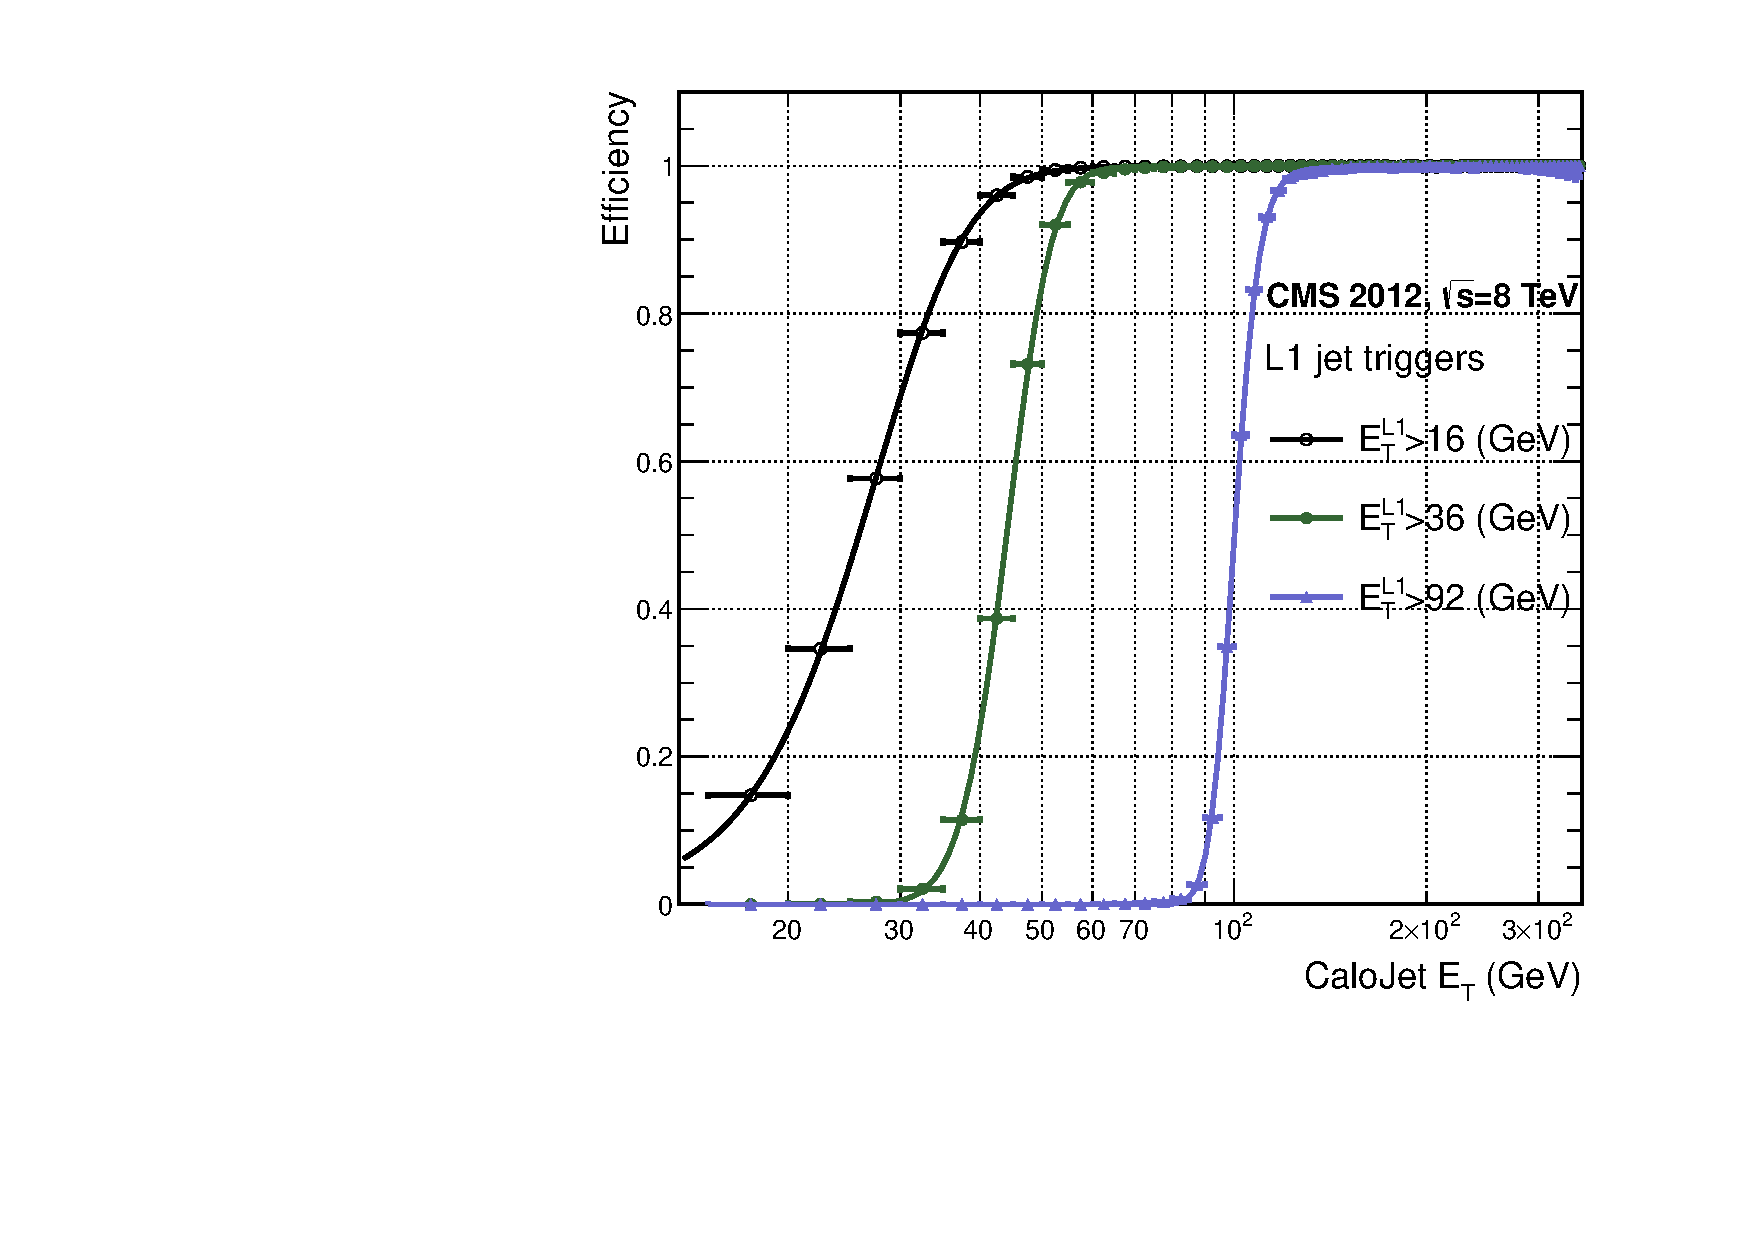
\includegraphics[width = 1.0\linewidth]{plots/jetpt_RunC.pdf}
\end{minipage}
\quad
\begin{minipage}[b]{0.48 \linewidth}
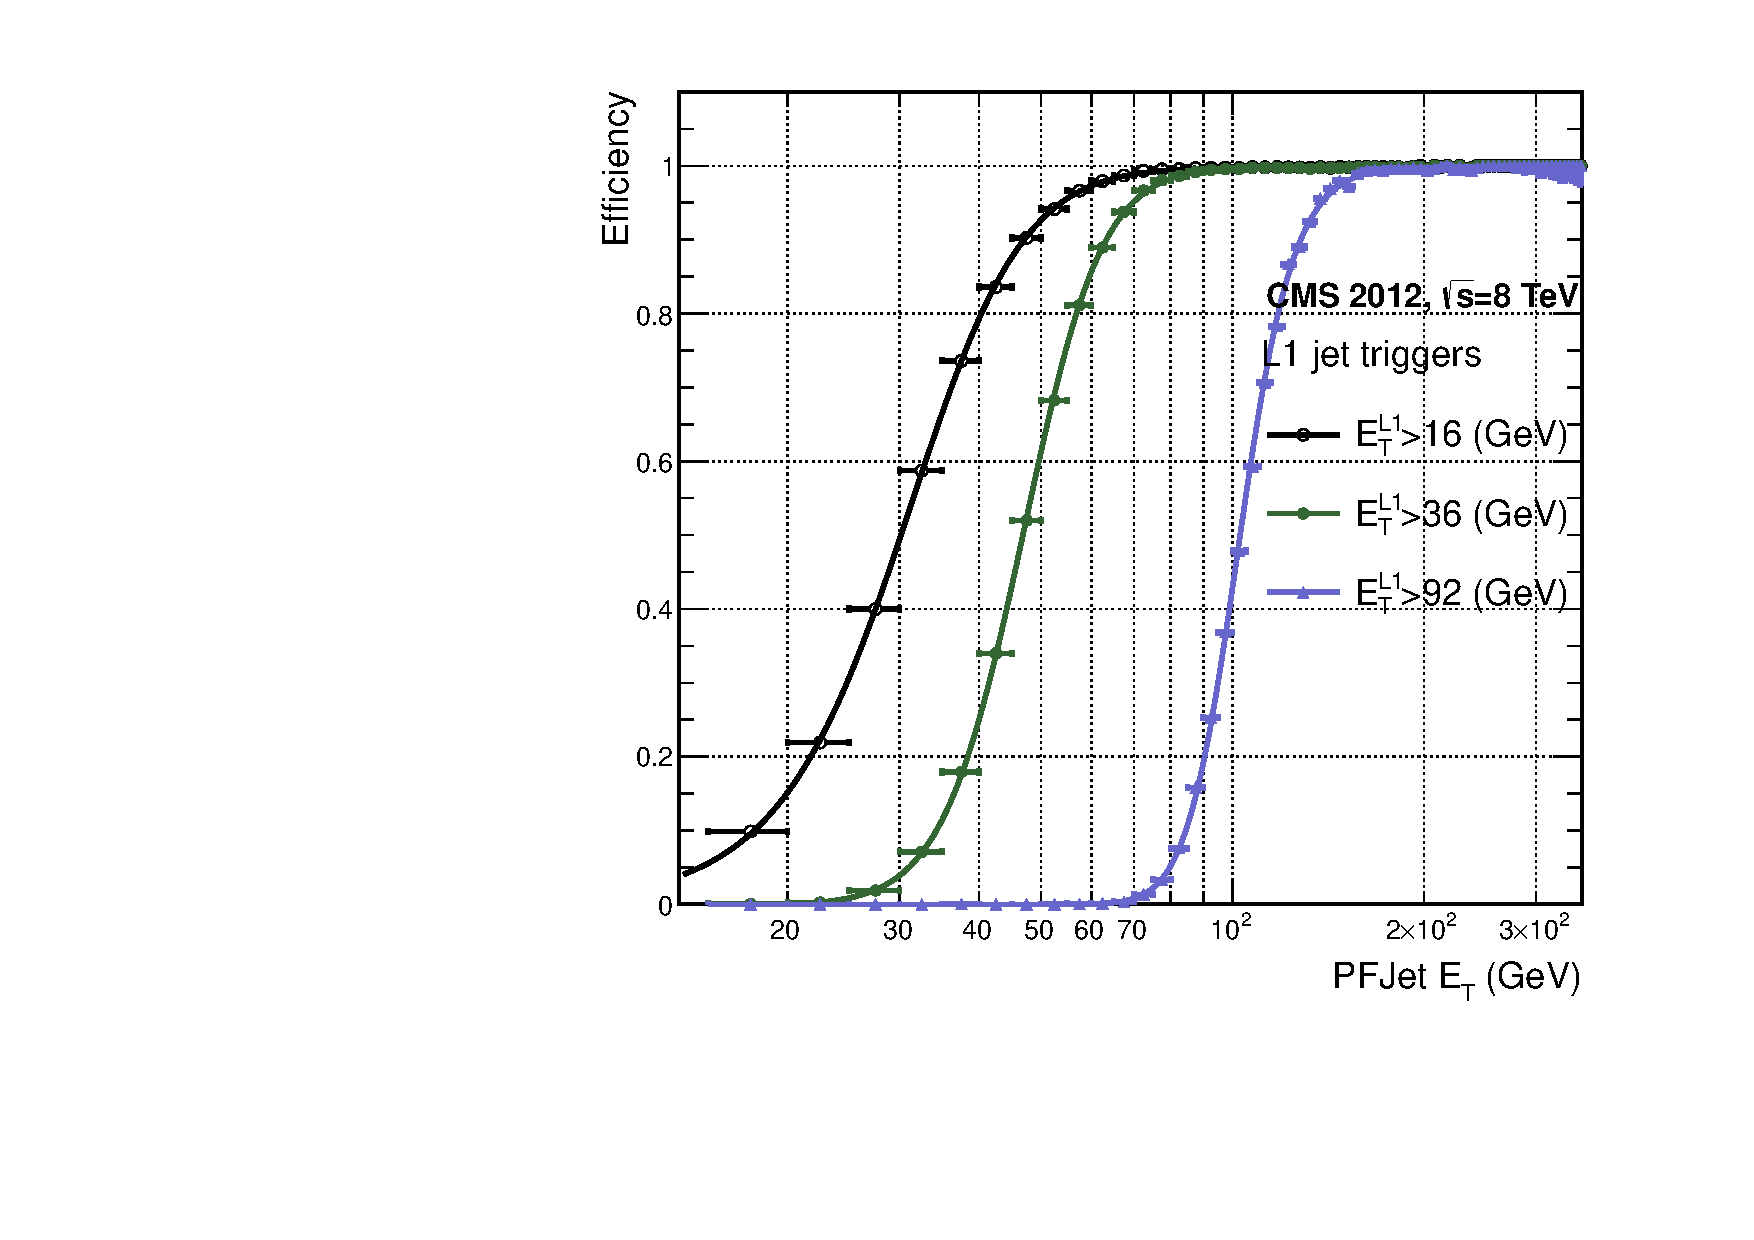
\includegraphics[width = 1.0\linewidth]{plots/jetpt_RunC_PF.pdf}
\end{minipage}
\quad
\caption[L1 jet efficiency turn-on curves as a function of the offline CaloJet and PFJet $\et$. ]{L1 jet efficiency turn-on curves as a function of the offline CaloJet $\et$ (left) and PFJet $\et$ (right), measured in 2012 Run Period C data and collected with an isolated single $\mu$ data sample.}
\label{fig:l1jet-calopf-mu} 

\end{figure}

\begin{table}
\begin{center}
\footnotesize
\begin{tabular*}{0.75\textwidth}{@{\extracolsep{\fill}}c|cc|cc}
\hline
\multicolumn{1}{c}{}& \multicolumn{2}{c}{Calo} & \multicolumn{2}{c}{PF} \\ 
\multicolumn{1}{c}{Trigger} & $\mu$ & \multicolumn{1}{c}{$\sigma$} & $\mu$ & $\sigma$ \\ \hline\hline
L1\_SingleJet16 & 21.09 $\pm$ 0.03 & 7.01 $\pm$ 0.02 & 22.17 $\pm$ 0.04 & 7.83 $\pm$ 0.03 \\ 
L1\_SingleJet36 & 41.15 $\pm$ 0.05 & 5.11 $\pm$ 0.02 & 39.16 $\pm$ 0.06 & 8.04 $\pm$ 0.03 \\ 
L1\_SingleJet92 & 95.36 $\pm$ 0.13 & 5.62 $\pm$ 0.03 & 90.85 $\pm$ 0.19 & 11.30 $\pm$ 0.10  \\ 
\end{tabular*}
\end{center}

\caption[Results of a cumulative \ac{EMG} function fit to the turn-on curves for \L1 single jet triggers in 2012 Run Period C.]{Results of a cumulative \ac{EMG} function fit to the turn-on curves for \L1 single jet triggers in run 2012 Run Period C, measured in an isolated $\mu$ data sample. The turn-on point, $\mu$, and resolution, $\sigma$, of the L1 jet triggers are measured with respect to offline Calo Jets (left) and PF Jets (right). }
\label{tab:l1jettable}
\end{table}

The results from the \L1 single jet triggers shows good performance for both \Calo and \PF jets. A better resolution for \Calo jets with respect to \L1 jets quantities is observed. This effect is due to \Calo jet reconstruction using the same detector systems as in \L1 jets, whereas  with \PF jet construction using tracker and muon information, a more smeared resolution when compared to \L1 is expected. 

\subsection{Effects of the \L1 jet seed}
\label{subsec:l1jetseedpu}

Between run period B and C of the 2012 data taking period, a jet seed threshold was introduced into the \L1 trigger jet algorithm. There was previously no direct requirement made on the energy deposited in the central region. The introduction of a jet seed threshold required that the central region have $\et \geq 5$\GeV, and was introduced to counteract the effects of high pile up running conditions which create a large number of soft non-collimated jets, that are then added to the jets from the primary interaction or other soft jets from other secondary interactions \cite{L1bryn}. This in turn causes a large increase in trigger rate due to the increase in the likelihood that the event causes the \L1 trigger to fire. This was implemented to maintain trigger thresholds by cutting the rate of events recorded without significant reduction in the efficiency of physics events of interest.

The effect of the introduction of this jet seed threshold between these two run periods is benchmarked through a comparison of the efficiency of the \L1 jet triggers with respect to offline Calo jets shown in Figure \ref{fig:l1jetseeds}, and the \L1 $H_{T}$ trigger efficiency in Figure \ref{fig:l1jetseedht} which is compared to offline $\theht$ constructed from Calo jets with $\et \geq$ 40\GeV. 

To negate any effects from different pile-up conditions in the run periods, the efficiencies are measured in events which contain between 15 and 20 primary vertices as defined in Appendix (\ref{app:primaryvertices}). 

\begin{figure}[ht]
\centering
\begin{minipage}[b]{0.48 \linewidth}
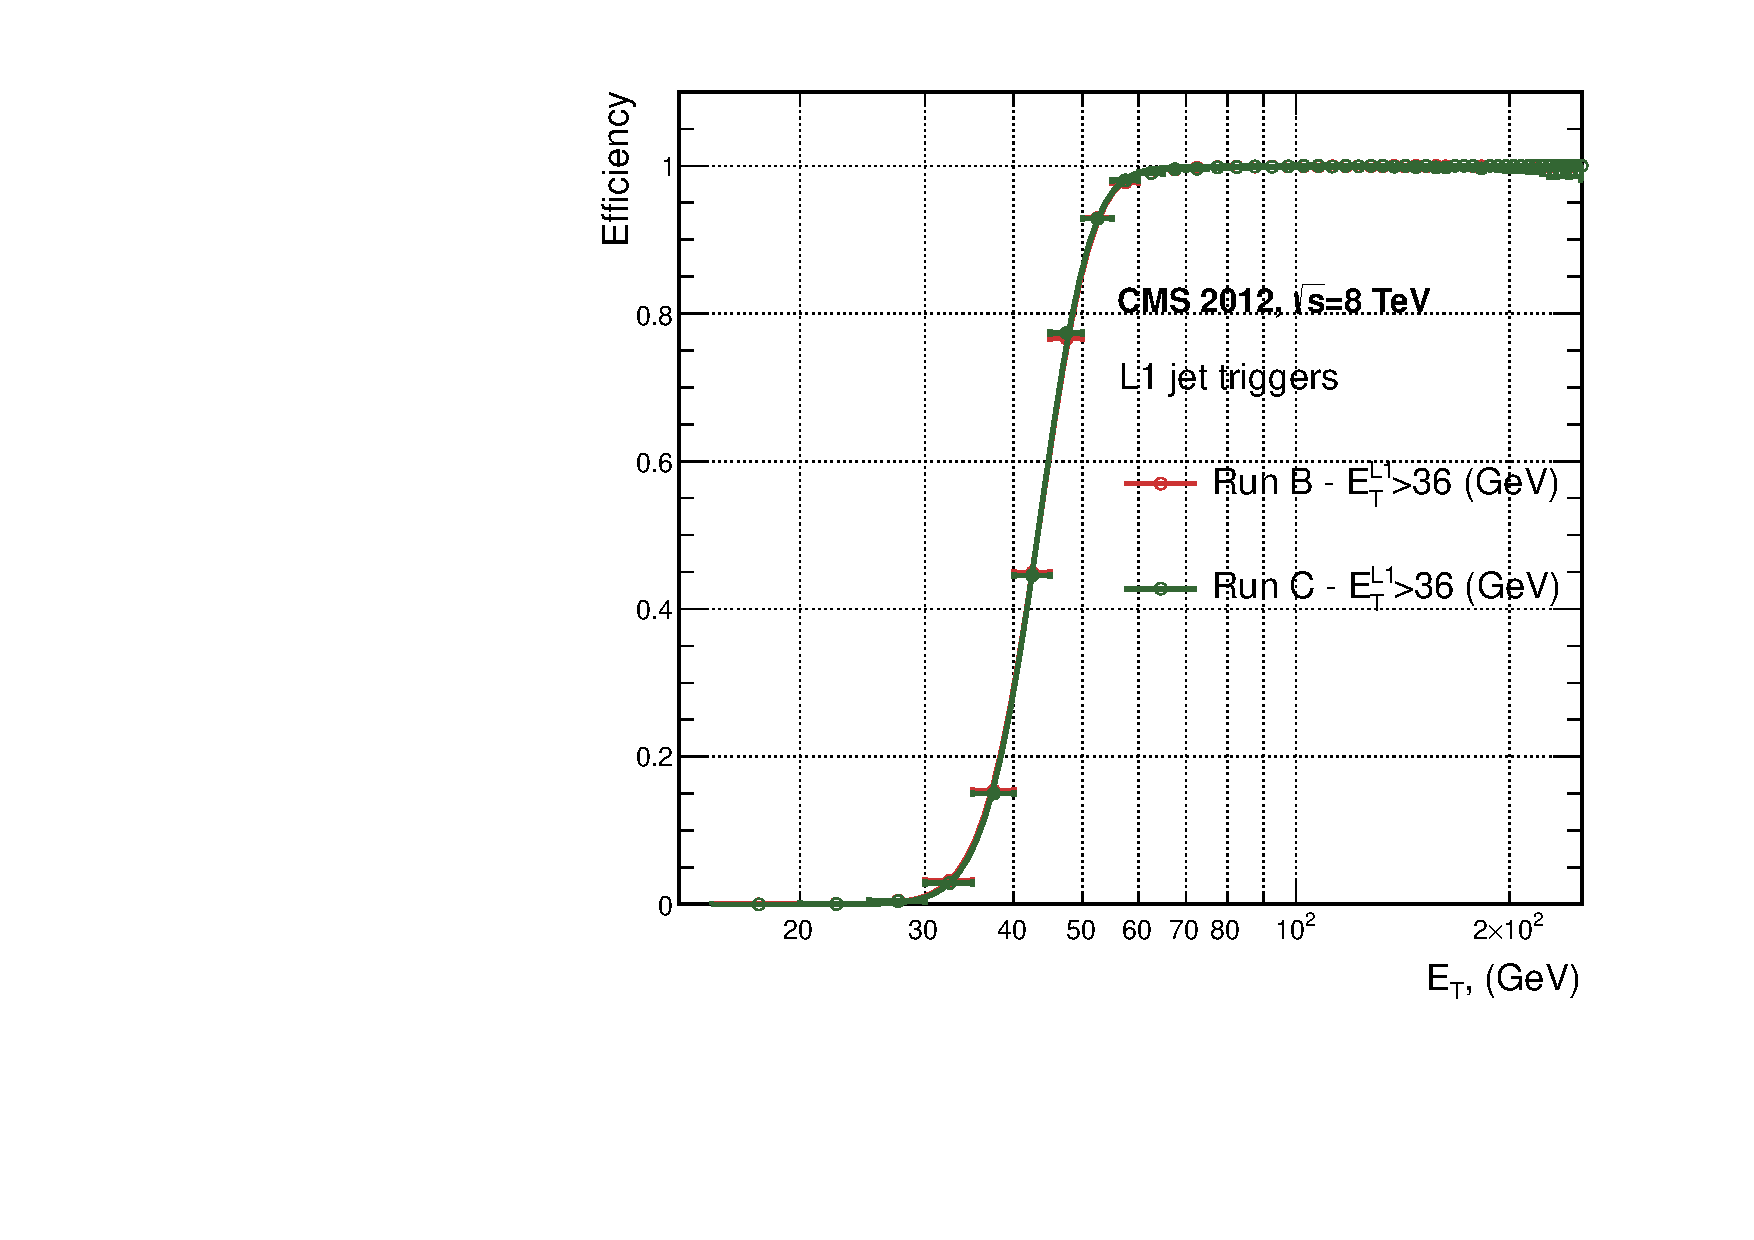
\includegraphics[width = 1.0\linewidth]{plots/jetseed_36.pdf}
\end{minipage}
\quad
\begin{minipage}[b]{0.48 \linewidth}
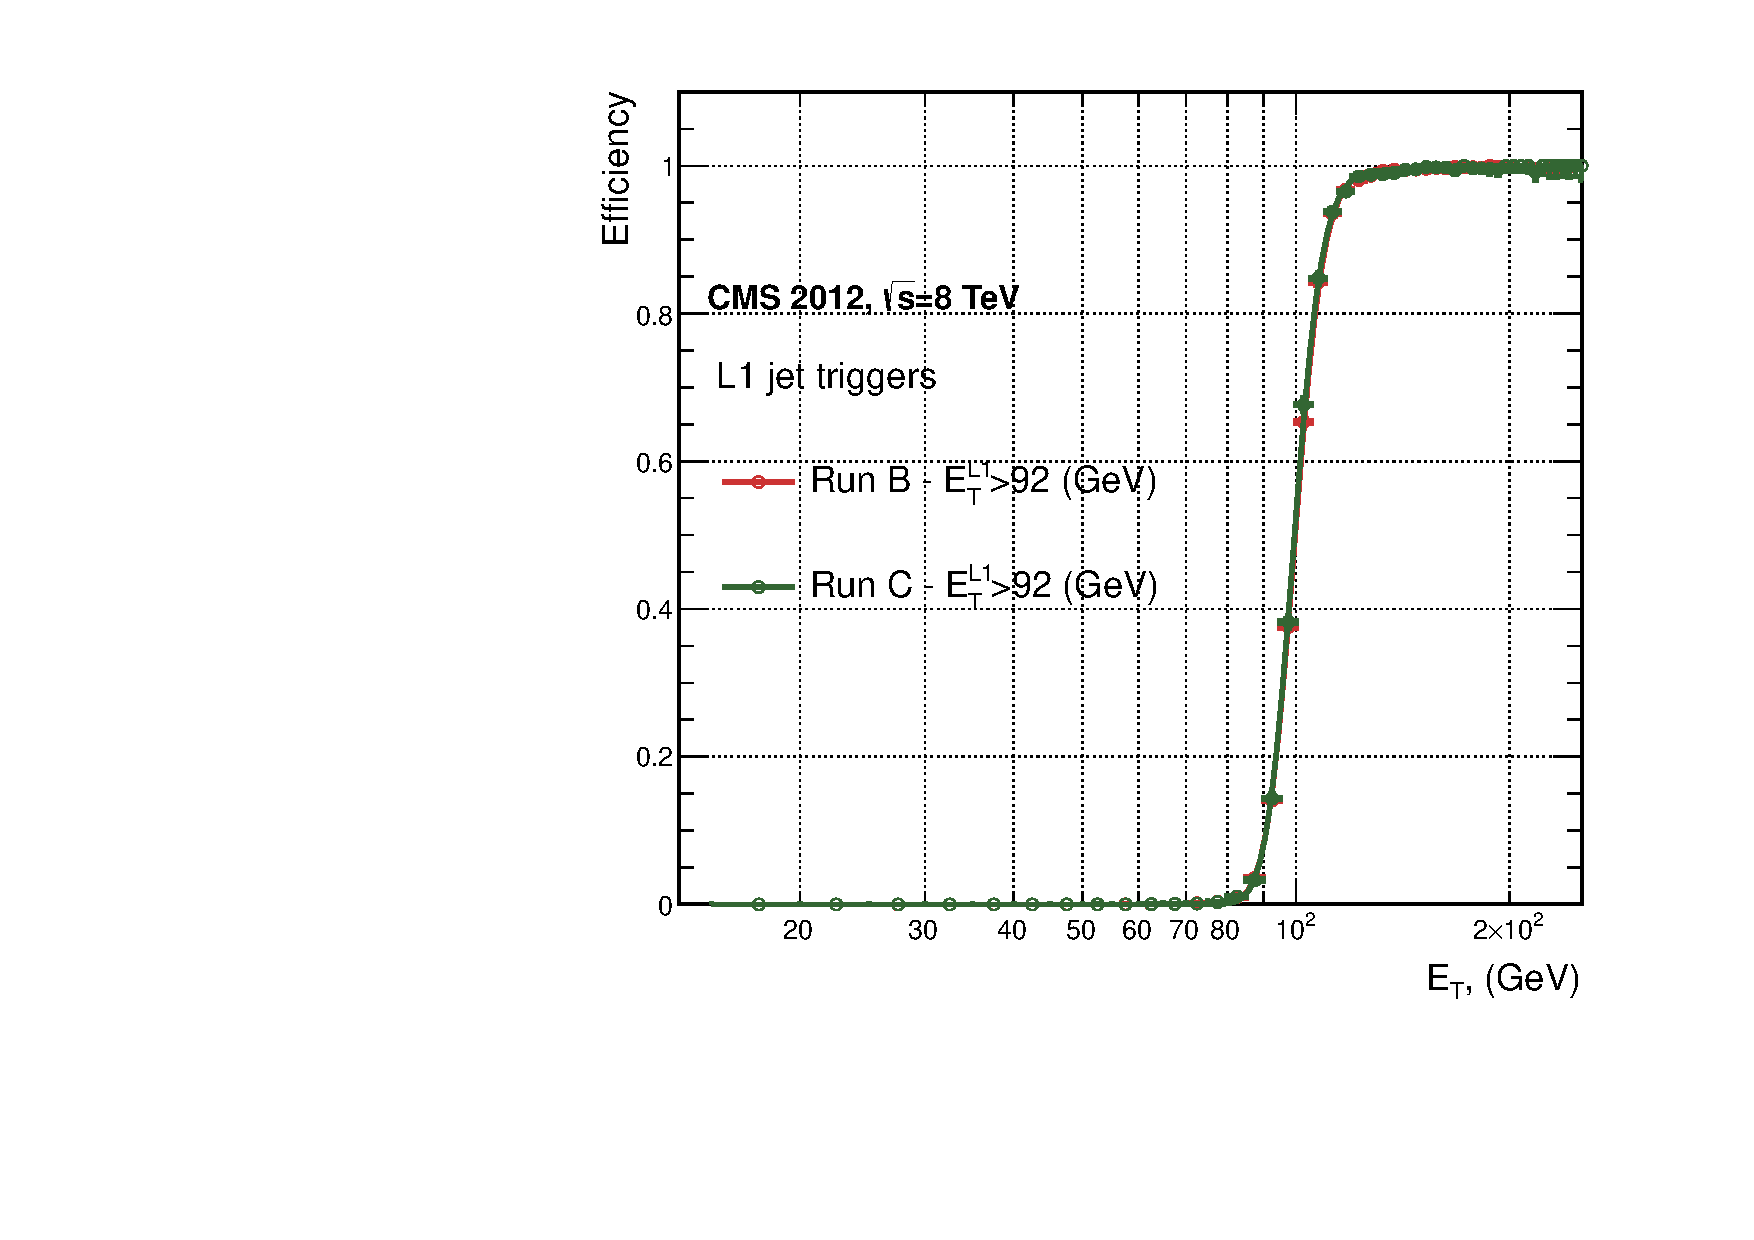
\includegraphics[width = 1.0\linewidth]{plots/jetseed_92.pdf}
\end{minipage}
\quad
\caption[L1 jet efficiency turn-on curves as a function of the offline CaloJet E$_{T}$ for the 2012 run period B and C.]{L1 jet efficiency turn-on curves as a function of the offline CaloJet E$_{T}$, measured for the \L1 SingleJet 36 and 92 trigger in 2012 run period B and C collected with an isolated single $\mu$' sample.}
\label{fig:l1jetseeds} 
\end{figure}

It can be seen that the performance of the $E_{T} > 36,92$ single jet are almost identical, with the jet seed having no measurable effect on these triggers as shown in Table \ref{tab:l1jetseedtable} . 

\begin{table}[h!]
\begin{center}
\footnotesize
\begin{tabular*}{0.75\textwidth}{@{\extracolsep{\fill}}c|cc|cc}
\hline
\multicolumn{1}{c}{}& \multicolumn{2}{c}{2012B} & \multicolumn{2}{c}{2012C} \\ 
\multicolumn{1}{c}{Trigger} & $\mu$ & \multicolumn{1}{c}{$\sigma$} & $\mu$ & $\sigma$ \\ \hline\hline
L1\_SingleJet36 & 40.29 $\pm$ 0.04& 5.34 $\pm$ 0.02 & 40.29 $\pm$ 0.11 & 5.21 $\pm$ 0.05 \\ 
L1\_SingleJet92 & 94.99 $\pm$ 0.09 & 5.93 $\pm$ 0.06 & 94.82 $\pm$ 0.29 & 5.74 $\pm$ 0.18 \\ 
\end{tabular*}
\end{center}
\caption[Results of a cumulative \ac{EMG} function fit to the turn-on curves for \L1 single jet triggers in the 2012 run period B and C.]{Results of a cumulative \ac{EMG} function fit to the turn-on curves for \L1 single jet triggers in the 2012 run period B and C, preselected on an isolated muon trigger. The turn-on point $\mu$ and resolution $\sigma$ of the L1 jet triggers are measured with respect to offline Calo Jets in run B (left) and run C (right). }
\label{tab:l1jetseedtable}

\end{table}

For the $\theht$ triggers, a large increase in rate during high pile-up conditions is expected. This is due to the low energy threshold required for a jet to be added to the \L1 $\theht$ sum, which is compiled from all uncorrected \L1 jets formed in the \RCT. The introduction of the jet seed threshold removes the creation of many of these soft low $\et$ jets, thus lowering the $\theht$ calculation at \L1. The effect on the trigger cross section for \L1 $\theht$ 150 trigger can be seen in Figure \ref{fig:l1rateplot}.

\begin{figure}[ht!]
\centering
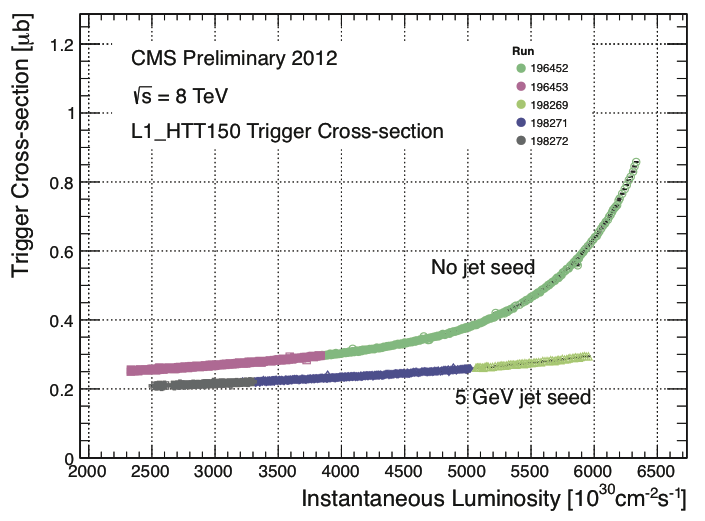
\includegraphics[scale=0.75]{plots/l1rateplot.pdf}
\caption[Trigger cross section for the L1HTT150 trigger path. ]{Trigger cross section for the L1HTT150 trigger path. Showing that a 5 \GeV jet seed threshold dramatically reduces the dependance of cross section on the instantaneous luminosity for \L1 $\theht$ triggers \cite{l1ratebrooke}.}  
\label{fig:l1rateplot}
\end{figure}  

Different behaviours for the trigger turn ons between these run periods are therefore expected. The turn on point is observed to shift to higher $\theht$ values after the introduction of the jet seed threshold, whilst having a sharper resolution due to less pile-up jets being included the $\theht$ sum. This effect is demonstrated in Table \ref{tab:l1jetseedtableHT}.

\begin{figure}[ht]
\centering
\begin{minipage}[b]{0.48 \linewidth}
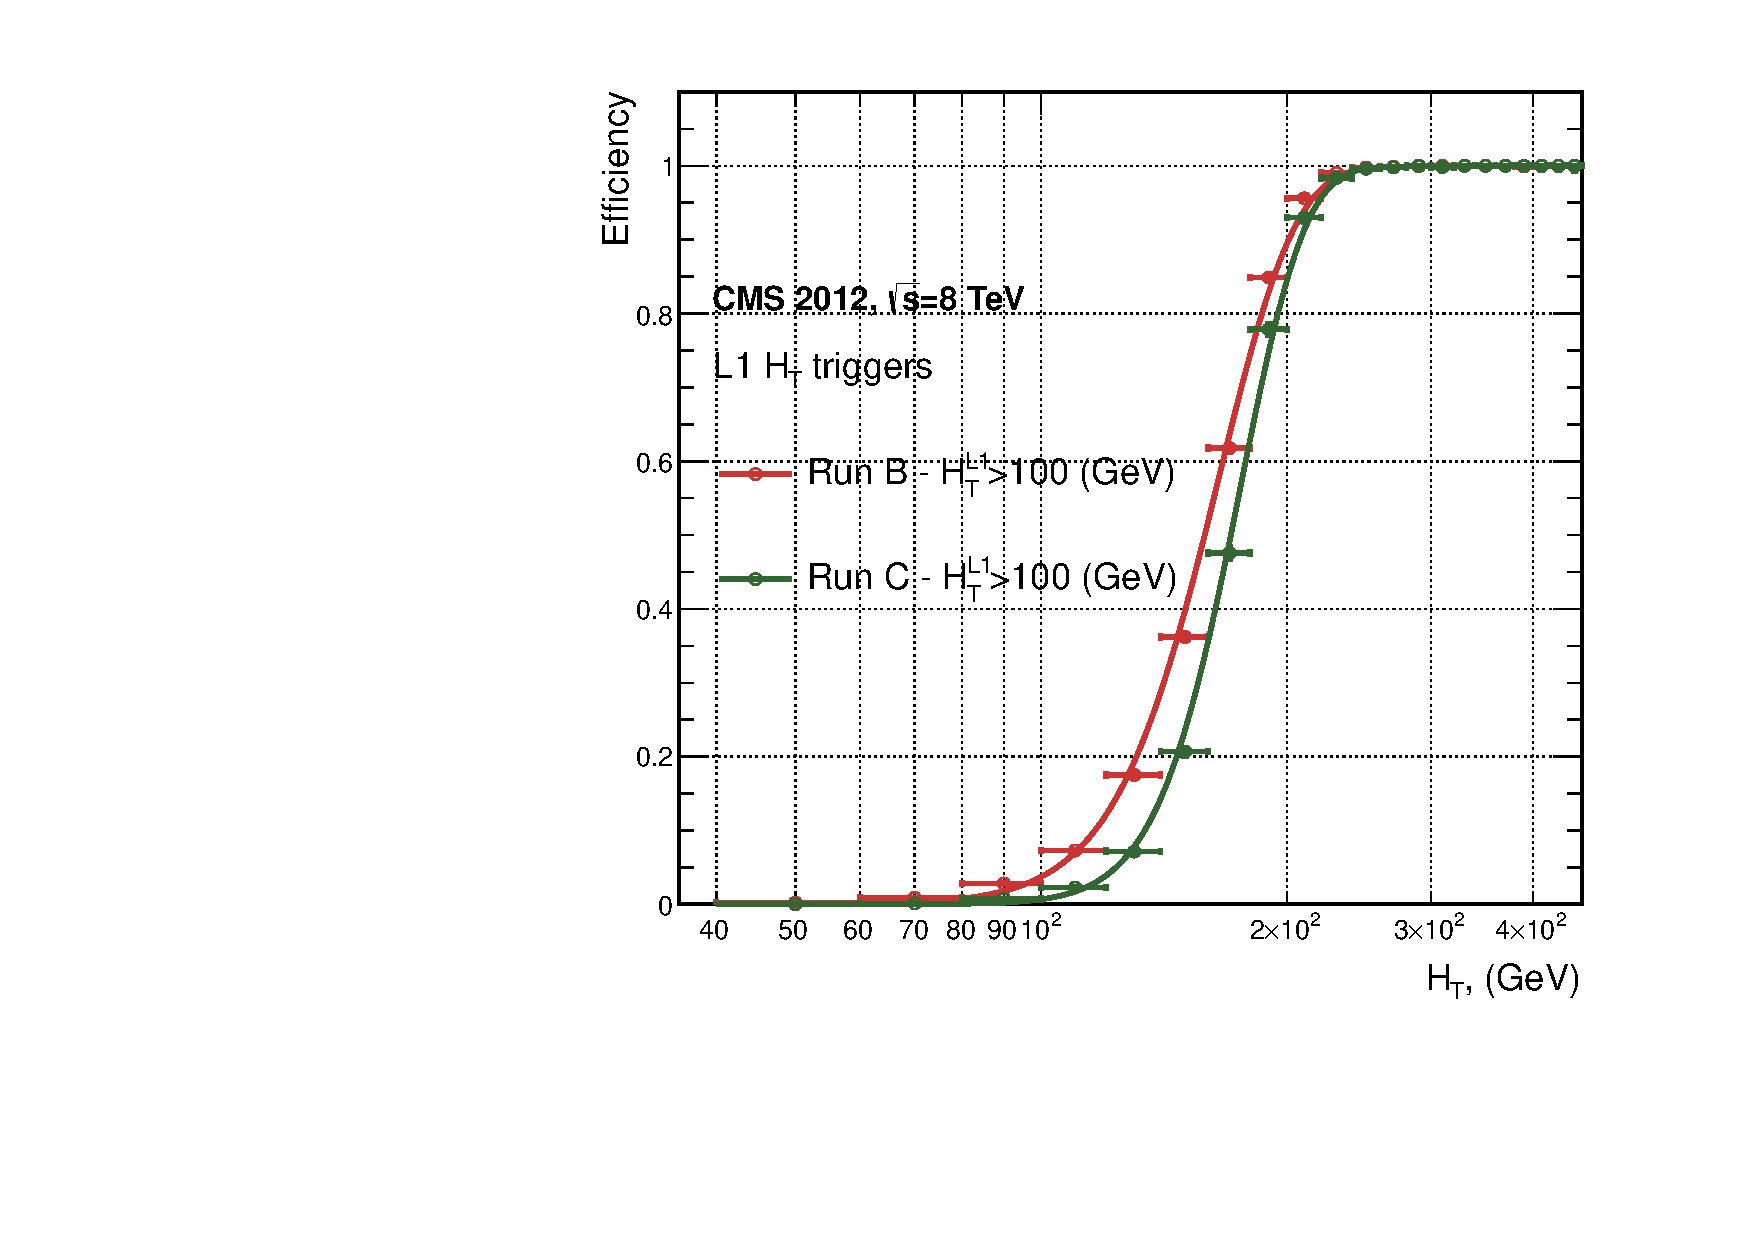
\includegraphics[width = 1.0\linewidth]{plots/jetseed_ht100.pdf}
\end{minipage}
\quad
\begin{minipage}[b]{0.48 \linewidth}
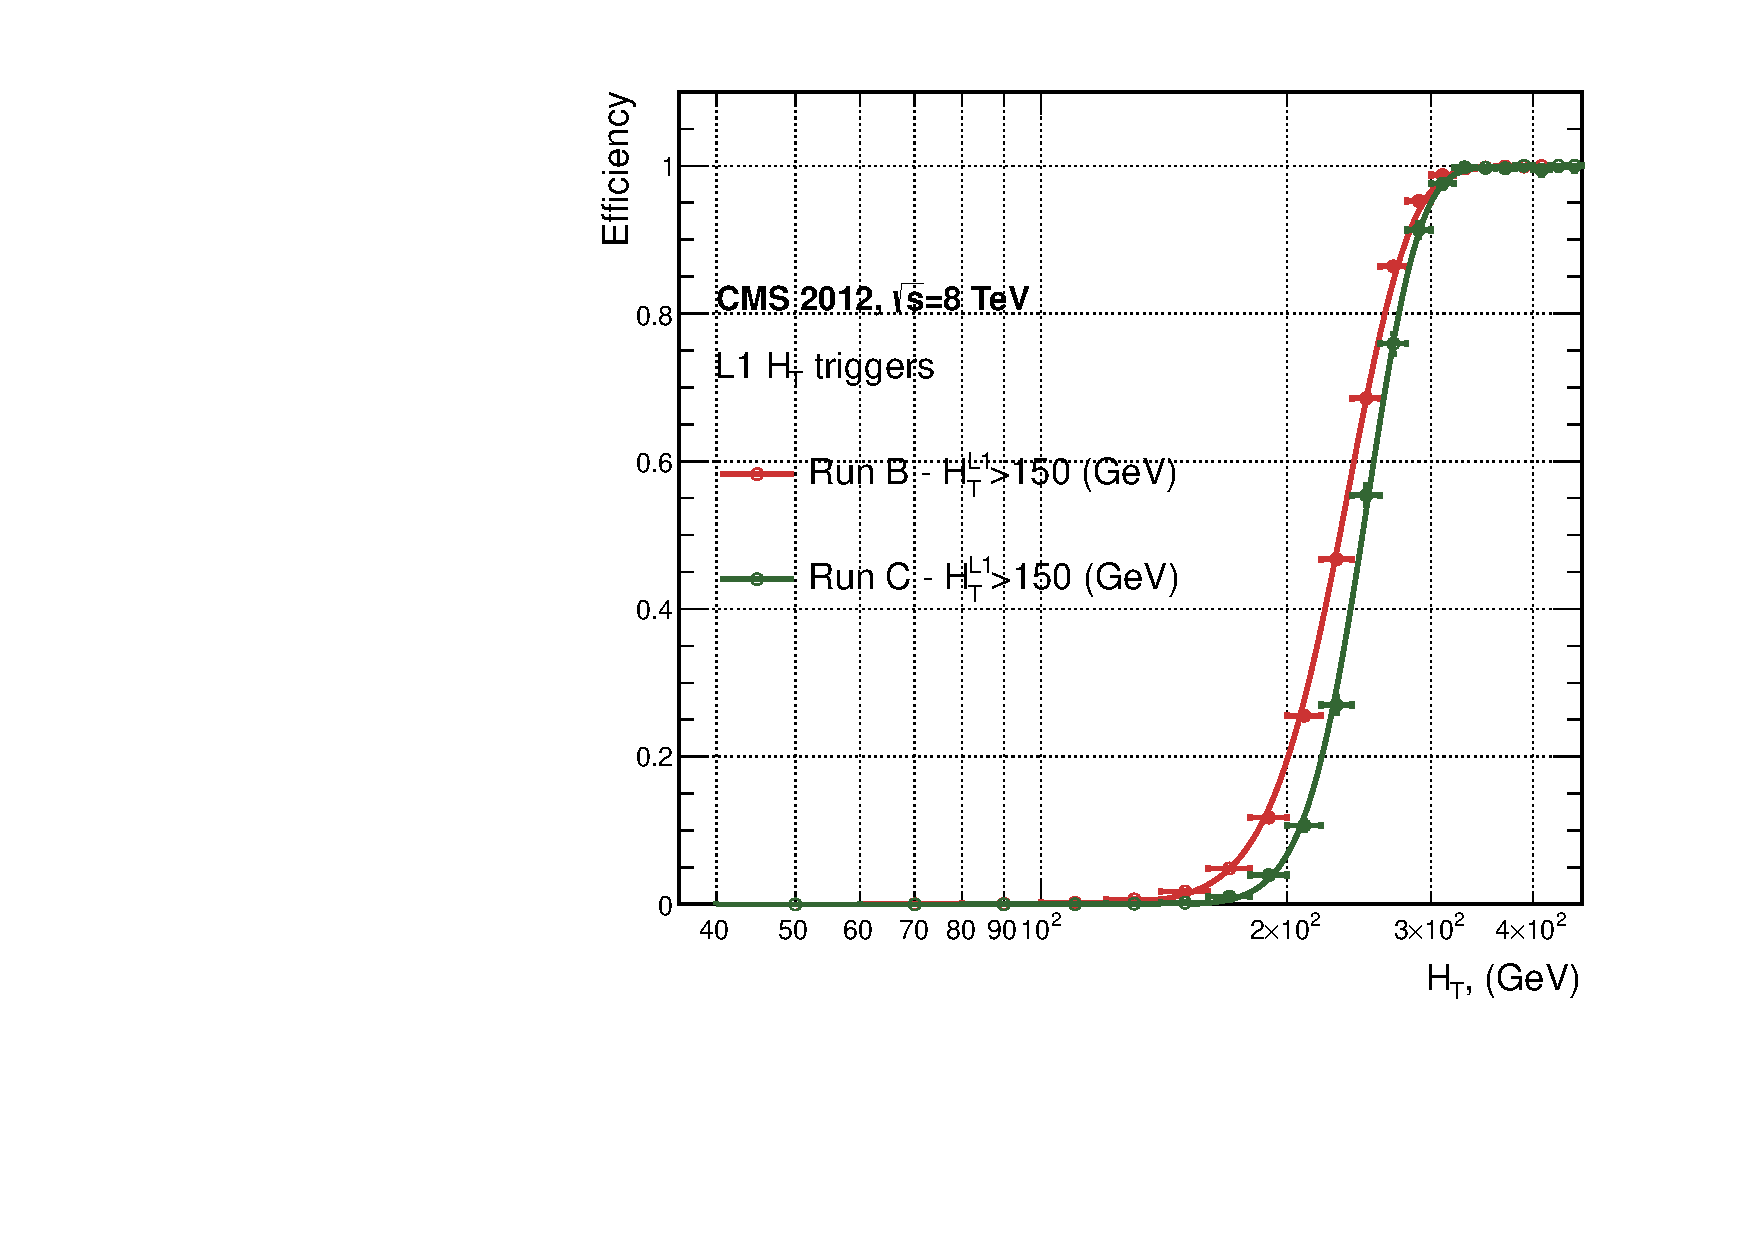
\includegraphics[width = 1.0\linewidth]{plots/jetseed_ht150.pdf}
\end{minipage}
\quad
\caption[\L1 $\theht$ efficiency turn-on curves as a function of the offline CaloJet $\theht$.]{\L1 $\theht$ efficiency turn-on curves as a function of the offline CaloJet $\theht$, measured for the \L1 $\theht$ 100 and 150 trigger during the run 2012 B and C collected using an isolated single $\mu$ triggered sample.}
\label{fig:l1jetseedht} 
\end{figure}


\begin{table}[h!]
\begin{center}
\footnotesize
\begin{tabular*}{0.75\textwidth}{@{\extracolsep{\fill}}c|cc|cc}
\hline
\multicolumn{1}{c}{}& \multicolumn{2}{c}{2012B} & \multicolumn{2}{c}{2012C} \\ 
\multicolumn{1}{c}{Trigger} & $\mu$ & \multicolumn{1}{c}{$\sigma$} & $\mu$ & $\sigma$ \\ \hline\hline
L1 HT-100 & 157.5 $\pm$ 0.08 & 32.9 $\pm$ 0.08 & 169.8 $\pm$ 0.08 & 28.7 $\pm$ 0.03 \\ 
L1 H1-150 & 230.9 $\pm$ 0.02 & 37.3 $\pm$ 0.01 & 246.4 $\pm$ 0.16 & 31.8 $\pm$ 0.05 \\ 
\end{tabular*}
\end{center}
\caption[Results of a cumulative \ac{EMG} function fit to the turn-on curves for $\theht$ in 2012 run period B and C.]{Results of a cumulative \ac{EMG} function fit to the turn-on curves for $\theht$ in run 2012 B and C, preselected on an isolated single $\mu$ trigger. The turn-on point $\mu$, resolution $\sigma$ of the \L1 $\theht$ triggers are measured with respect to offline $\theht$ formed from CaloJets with a $\et \geq 40$  in run period B (left) and C (right). }
\label{tab:l1jetseedtableHT}
\end{table}

\subsection{Robustness of \L1 jet performance against pile-up}
\label{subsec:l1jetpu}

The performance of the L1 single jet triggers is evaluated in different pile-up conditions to benchmark any dependence on pile-up. Three different pile-up bins of 0-10, 10-20 and $>$20 vertices are
defined, reflecting the low, medium and high pile-up running conditions at \CMS in 2012. This is benchmarked relative to \Calo and \PF jets for the run 2012 C period where the jet seed threshold is applied, with \L1 single jet thresholds of 16, 36 and 92 \GeV, shown in Figure \ref{fig:l1jet-calopf-pu}. The results of fits to these efficiency turn-on curves are given in Table \ref{tab:l1jcaloputable} and Table \ref{tab:l1pfputable} for \Calo and \PF jets respectively.



\begin{figure}[ht]
\centering
\begin{minipage}[b]{0.48 \linewidth}
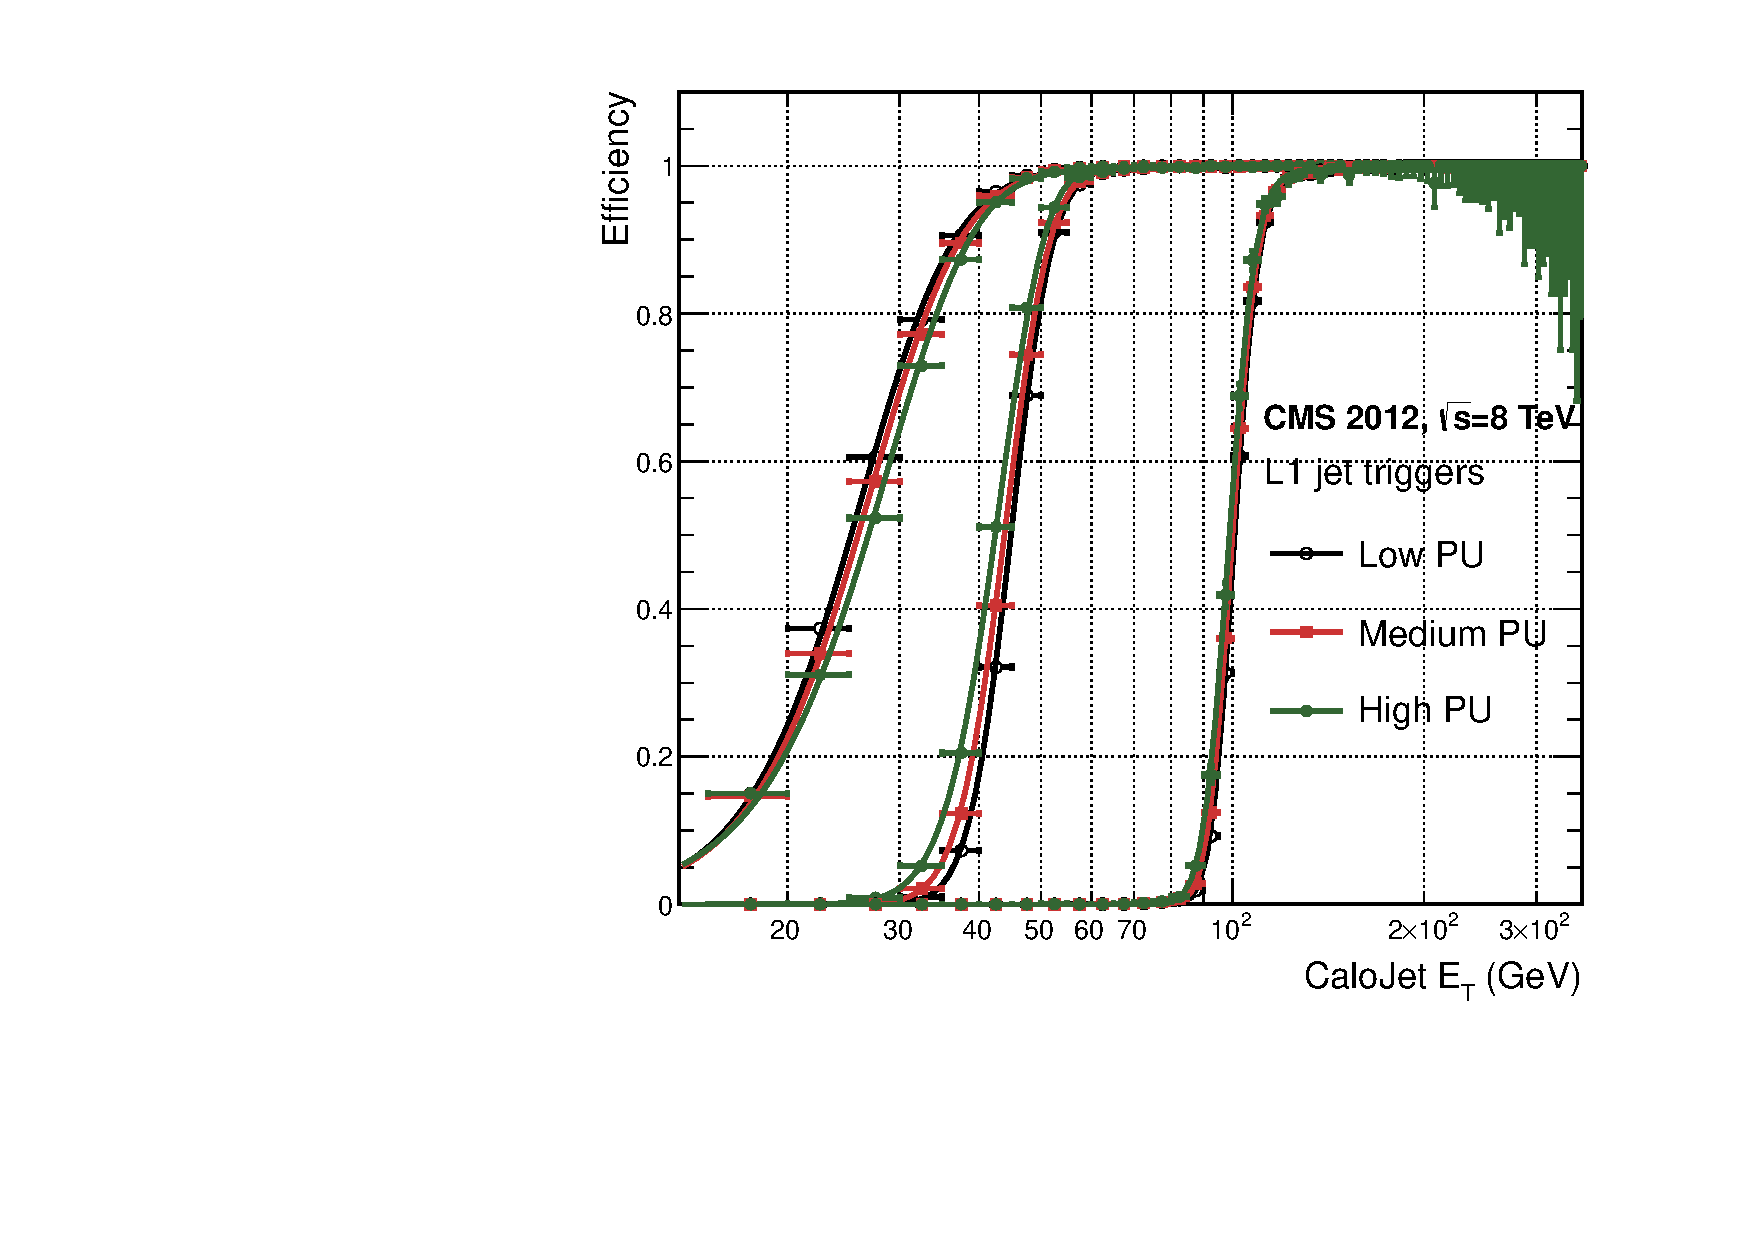
\includegraphics[width = 1.0\linewidth]{plots/jetpt_RunC_calopu.pdf}
\end{minipage}
\quad
\begin{minipage}[b]{0.48 \linewidth}
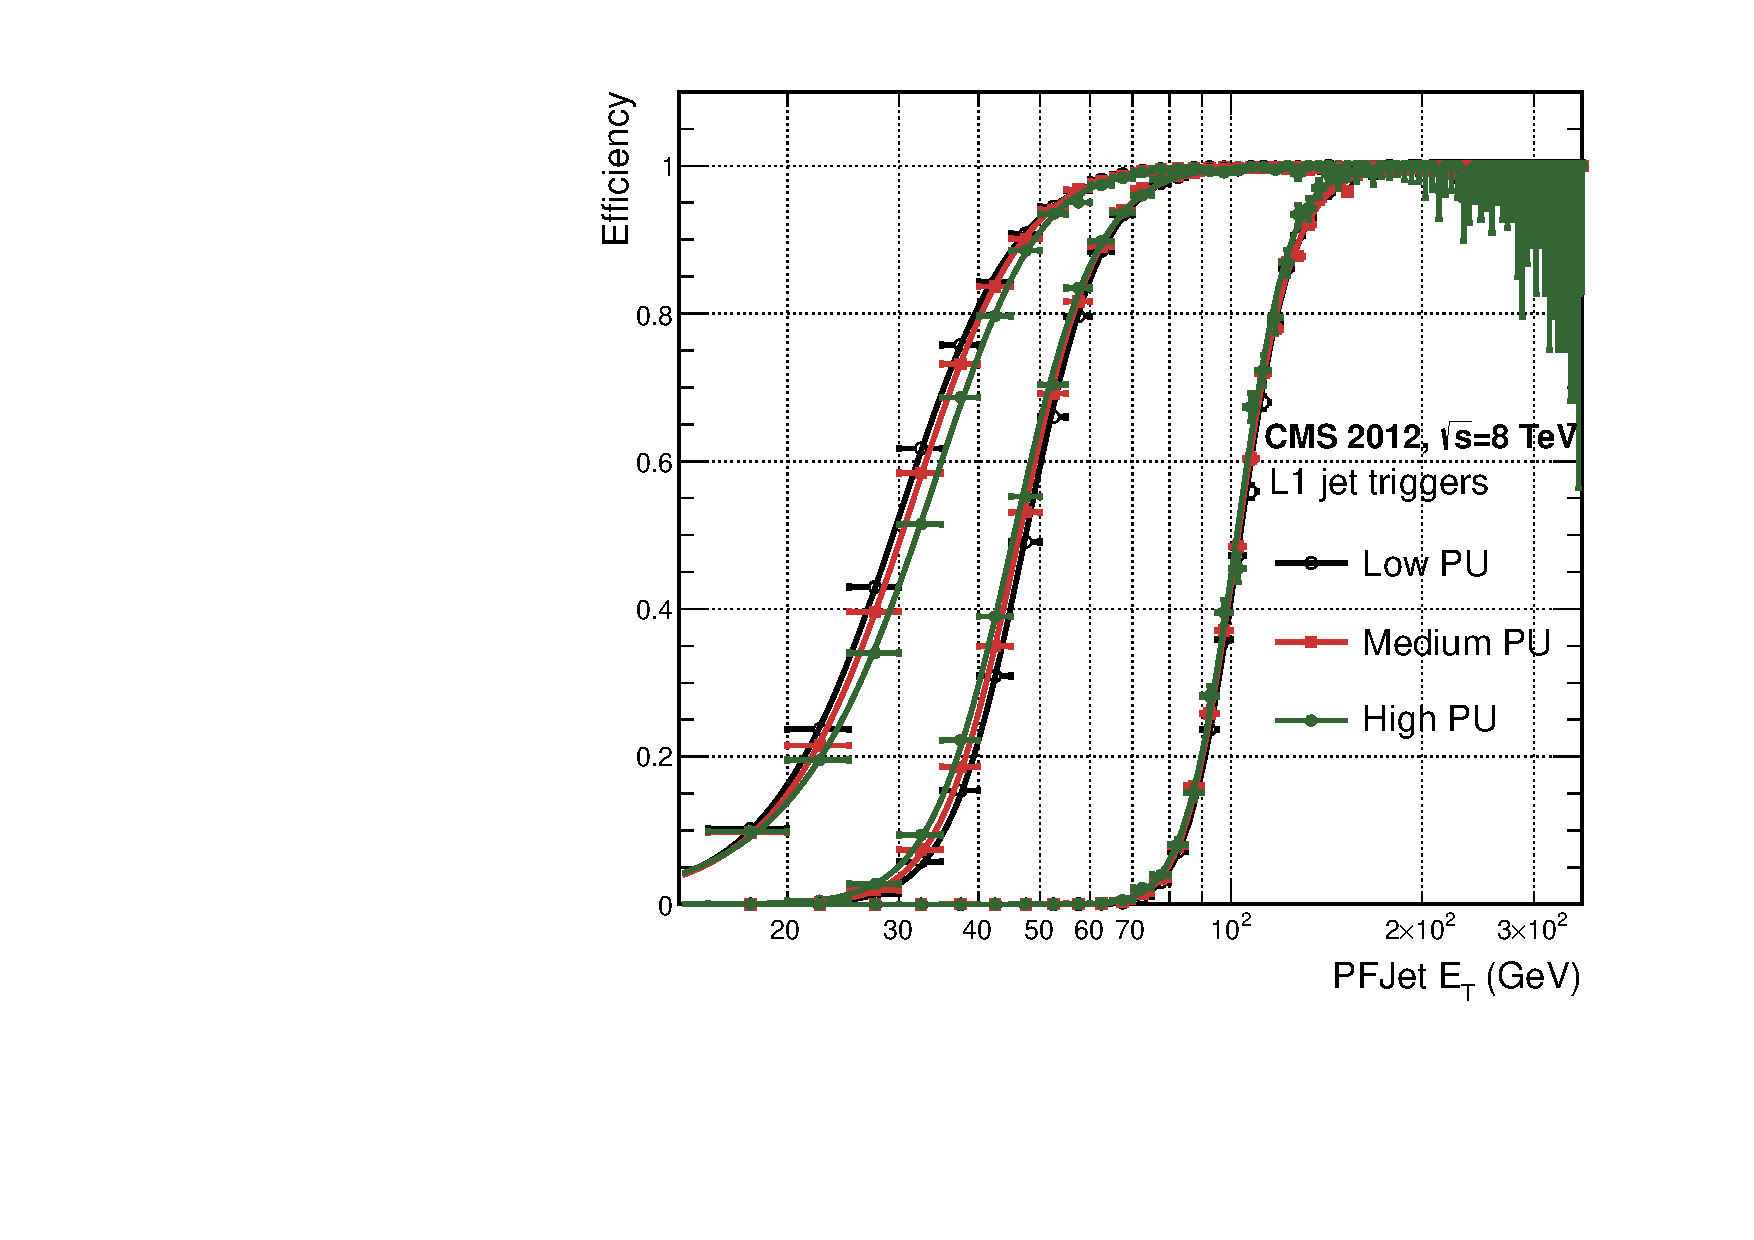
\includegraphics[width = 1.0\linewidth]{plots/jetpt_RunC_pfpu.pdf}
\end{minipage}
\quad
\caption[\L1 jet efficiency turn-on curves as a function of the leading offline $\et$ \Calo (left) and \PF (right) jet, for low, medium and high pile-up conditions.]{\L1 jet efficiency turn-on curves as a function of the leading offline $\et$\Calo (left) and \PF (right) jet, for low, medium and high pile-up conditions.}
\label{fig:l1jet-calopf-pu} 
\end{figure}



\begin{table}[ht]
%\begin{center}
\footnotesize
\begin{tabular*}{1.0\textwidth}{@{\extracolsep{\fill}}c|cc|cc|cc}
\hline
\multicolumn{1}{c}{Vertices} & \multicolumn{2}{c}{ 0-10 } & \multicolumn{2}{c}{11-20} & \multicolumn{2}{c}{$>$ 20}   \\ 
\multicolumn{1}{c}{} & $\mu$ & \multicolumn{1}{c}{$\sigma$} & $\mu$ & \multicolumn{1}{c}{$\sigma$} & $\mu$ & $\sigma$ \\ \hline\hline
L1\_SingleJet16 & 19.9 $\pm$ 0.1 & 6.1 $\pm$ 0.3  & 20.8 $\pm$ 0.1 & 6.5 $\pm$ 0.1 & 22.3 $\pm$ 0.2 & 7.5 $\pm$ 0.1\\ 
L1\_SingleJet36 & 41.8 $\pm$ 0.1 & 4.6 $\pm$ 0.1 & 40.9 $\pm$ 0.1 & 5.1 $\pm$ 0.1 & 40.6 $\pm$ 0.6 & 5.9 $\pm$ 0.2 \\ 
L1\_SingleJet92 & 95.9 $\pm$ 0.2 & 5.4 $\pm$ 0.1 & 95.2 $\pm$ 0.2 & 5.6 $\pm$ 0.1 & 94.5 $\pm$ 0.6 & 6.2 $\pm$ 0.3  \\ 
\end{tabular*}
%\end{center}
\caption[Results of a cumulative \ac{EMG} function fit to the efficiency turn-on curves for \L1 single jet triggers in the 2012 run period C, for low,medium and high pile-up conditions.]{Results of a cumulative \ac{EMG} function fit to the efficiency turn-on curves for \L1 single jet triggers in the 2012 run period C,  measured from isolated $\mu$ triggered data. The turn-on point, $\mu$, and resolution, $\sigma$, of the \L1 jet triggers are measured with respect to offline \Calo jets in low (left), medium (middle) and high (right) pile-up conditions. }
\label{tab:l1jcaloputable}
\end{table}

\begin{table}[ht]
%\begin{center}
\footnotesize
\begin{tabular*}{1.0\textwidth}{@{\extracolsep{\fill}}c|cc|cc|cc}
\hline
 \multicolumn{1}{c}{Vertices} & \multicolumn{2}{c}{ 0-10 } & \multicolumn{2}{c}{11-20} & \multicolumn{2}{c}{$>$ 20}   \\ 
 \multicolumn{1}{c}{} & $\mu$ & \multicolumn{1}{c}{$\sigma$} & $\mu$ & \multicolumn{1}{c}{$\sigma$} & $\mu$ & $\sigma$ \\ \hline\hline
L1\_SingleJet16 & 21.1 $\pm$ 0.1 & 7.16 $\pm$ 0.05 & 22.34 $\pm$ 0.1 & 7.9 $\pm$ 0.1 & 24.6 $\pm$ 0.2 & 9.5 $\pm$ 0.1 \\ 
L1\_SingleJet36 & 39.6 $\pm$ 0.1 & 7.4 $\pm$ 0.1 & 38.4 $\pm$ 0.1  & 7.4 $\pm$ 0.1 & 37.1 $\pm$ 0.2 & 7.5 $\pm$ 0.1 \\ 
L1\_SingleJet92 & 91.6 $\pm$ 0.3 & 11.3 $\pm$ 0.2 & 90.4 $\pm$ 0.3 & 11.2 $\pm$ 0.1 & 92.0 $\pm$ 0.9 & 12.1 $\pm$ 0.4  \\ 
\end{tabular*}
%\end{center}
\caption[Results of a cumulative \ac{EMG} function fit to the efficiency   turn-on curves for Level-1 single jet triggers in the 2012 run period C, for low,medium and high pile-up conditions.]{Results of a cumulative \ac{EMG} function fit to the efficiency   turn-on curves for Level-1 single jet triggers in the 2012 run period C, measured from isolated $\mu$ triggered data. The turn-on point, $\mu$, and resolution, $\sigma$, of the \L1 jet triggers are measured with respect to offline \PF jets in low (left), medium (middle) and high (right) pile-up conditions. }
\label{tab:l1pfputable}
\end{table}

No significant drop in efficiency is observed in the presence of a high number of primary vertices. The increase in hadronic activity in higher pile-up conditions, combined with the absence of pile-up subtraction for L1 jets, results in the expected observation of a decrease in the $\mu$ value of the efficiency turn-ons as a function of pile-up, while the resolution, $\sigma$ of the turn-ons are found to gradually worsen as expected with increasing pile-up.

These features are further emphasised when shown as a function of

\begin{equation}
\frac{(\text{L1 E}_{T} -  \text{Offline E}_{T})}{\text{Offline E}_{T}}
\label{eq:jetresolution}
\end{equation}

in bins of matched leading offline jet $\et$, of which the individual fits can be found in Appendix (\ref{app:jetpuresolution}).  Each of these distributions are fitted with an \ac{EMG} function as defined in Equation (\ref{eq:emg}).

The $\mu$, $\sigma$ and $\lambda$ values extracted for the low, medium and high pile-up conditions are shown for Calo and PF jets in Figure \ref{fig:jetptresultspu} and Figure \ref{fig:pfjetptresultspu} respectively. The central value of $\frac{(\text{L1 E}_{T} -  \text{Offline E}_{T})}{\text{Offline E}_{T}}$ is observed to increases as a function of jet $\et$, whilst the resolution is also observed to improve at higher offline jet $\et$. 

\begin{figure}[h!]
  \vspace{20pt}
	\centering
	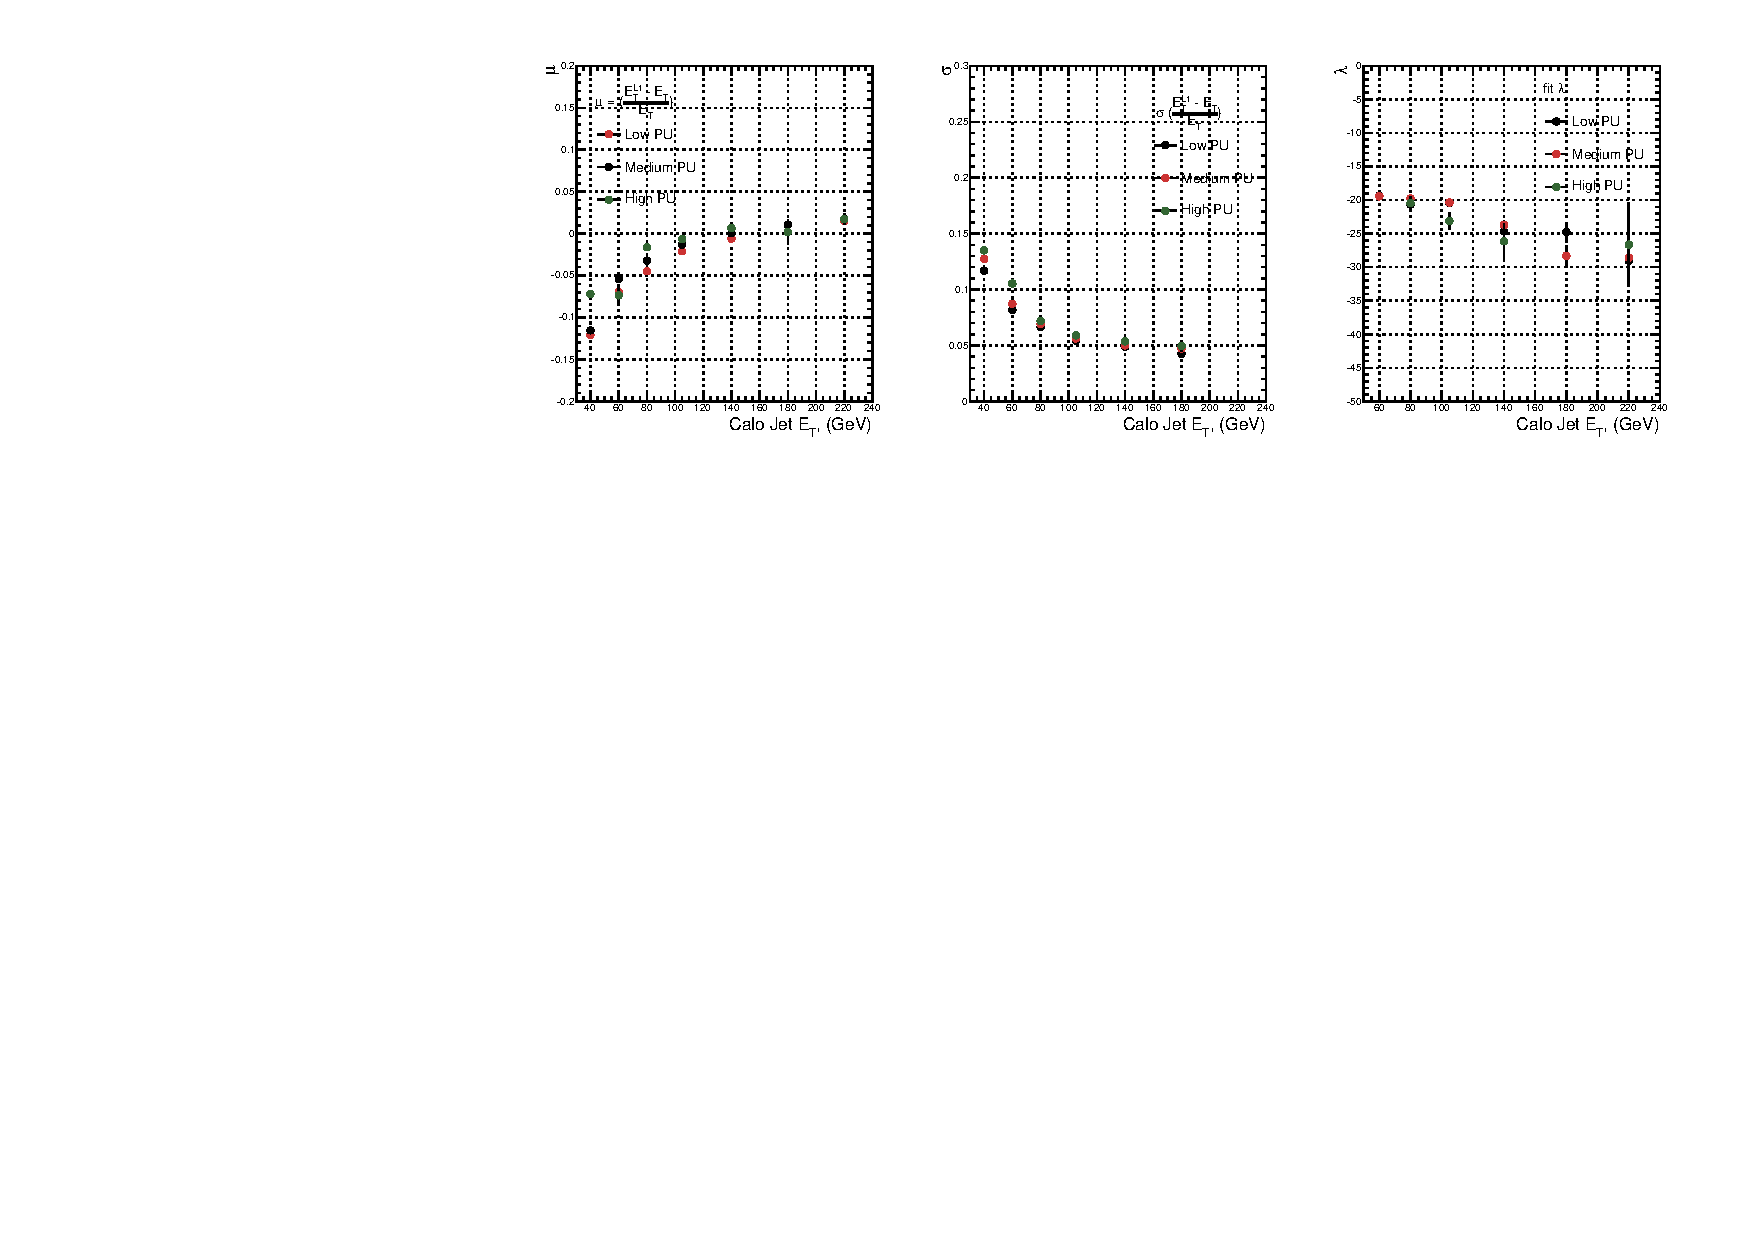
\includegraphics[width=1.0\textwidth]{plots/res_CaloJet_summary.pdf}
	\caption[Fit values from an \ac{EMG} function fitted to the resolution plots of leading Calo jet $\et$ measured as a function of  $\frac{(\text{L1 E}_{T} -  \text{Offline E}_{T})}{\text{Offline E}_{T}}$ for low, medium and high pile-up conditions. ]{Fit values from an \ac{EMG} function fitted to the resolution plots of leading Calo jet $\et$ measured as a function of  $\frac{(\text{L1 E}_{T} -  \text{Offline E}_{T})}{\text{Offline E}_{T}}$ for low, medium and high pile-up conditions. The plots show the mean $\mu$ (left), resolution $\sigma$ (middle) of the Gaussian as well as the decay term $\lambda$ (right) of the exponential.}
	\label{fig:jetptresultspu}
\end{figure}

\begin{figure}[h!]
  \vspace{20pt}
        \centering
        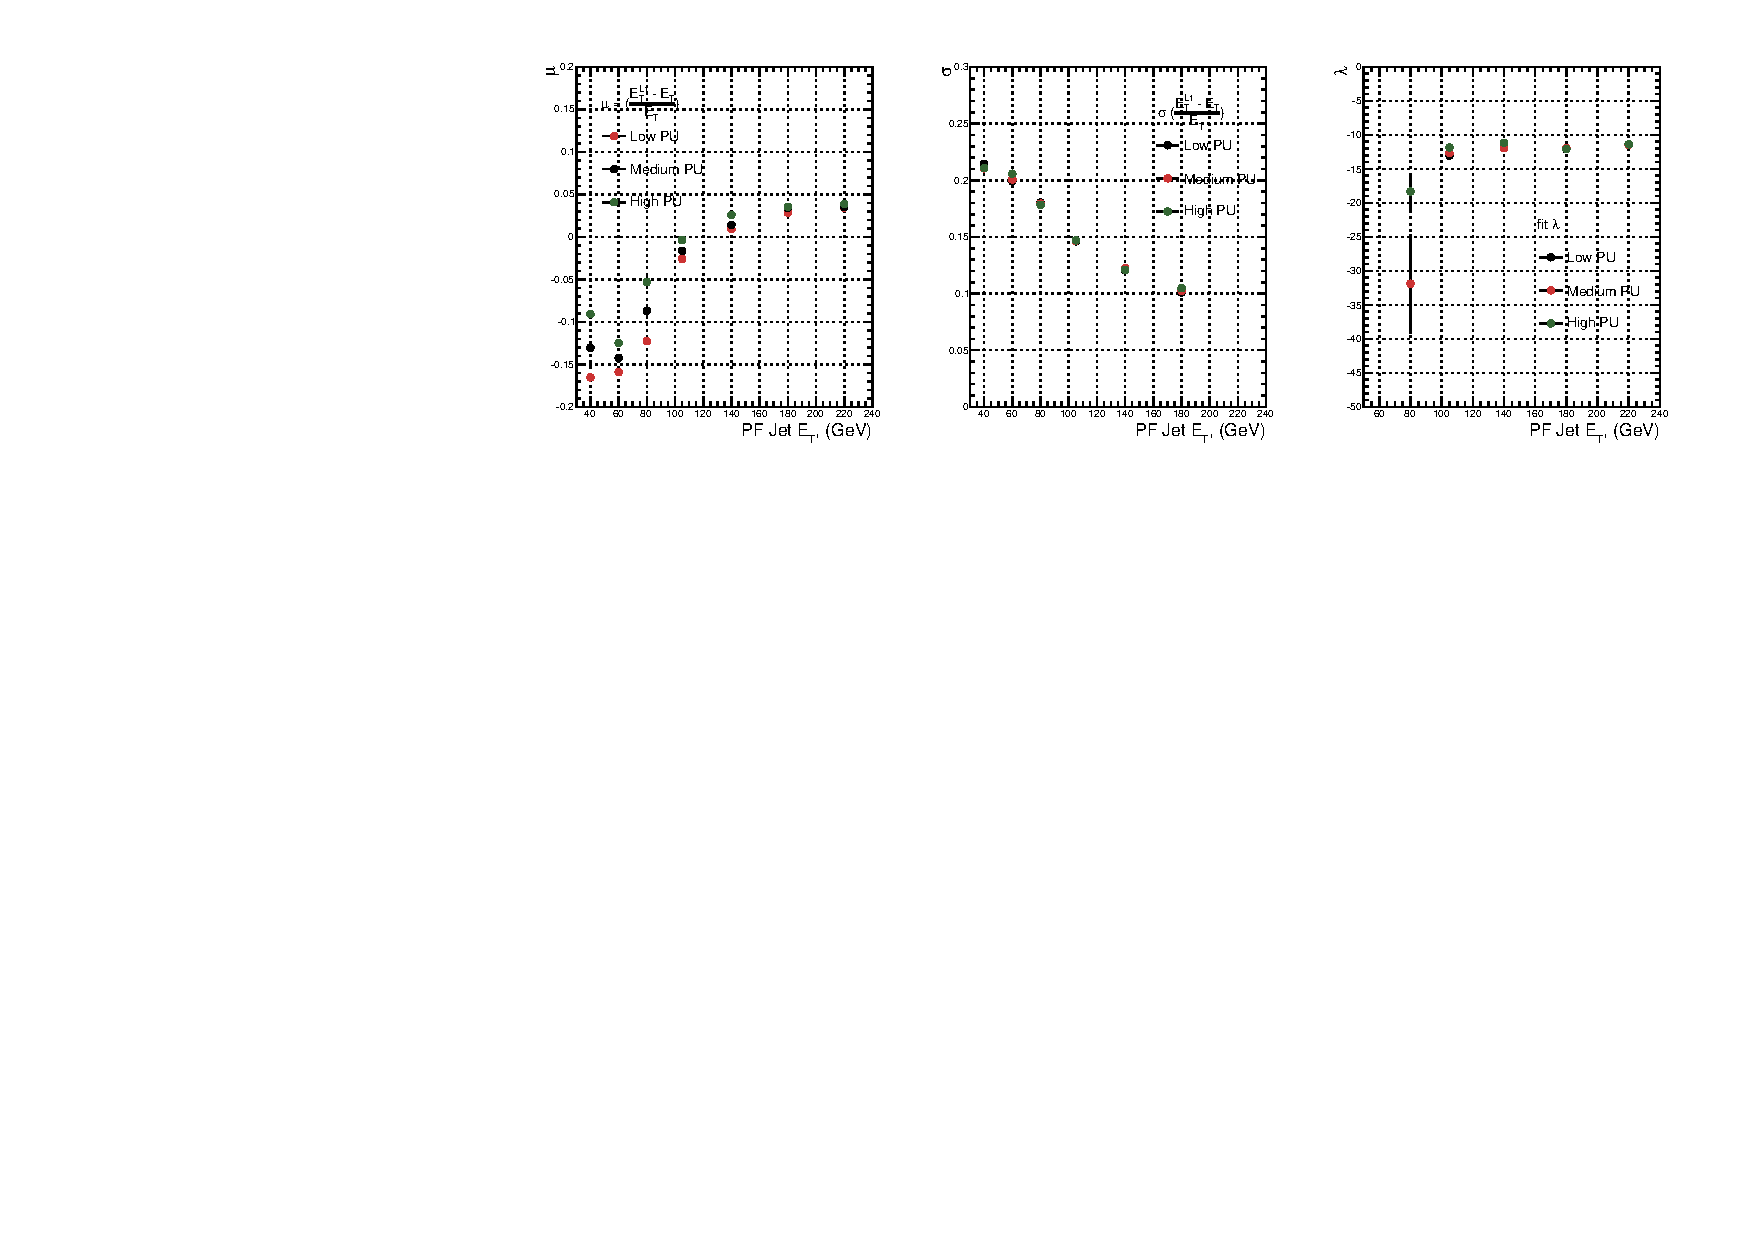
\includegraphics[width=1.0\textwidth]{plots/res_PFJet_summary.pdf}
        \caption[Fit values from an \ac{EMG} function fitted to the resolution plots of leading PF jet $\et$ measured as a function of  $\frac{(\text{L1 E}_{T} -  \text{Offline E}_{T})}{\text{Offline E}_{T}}$ for low, medium and high pile-up conditions.]{Fit values from an \ac{EMG} function fitted to the resolution plots of leading PF jet $\et$ measured as a function of  $\frac{(\text{L1 E}_{T} -  \text{Offline E}_{T})}{\text{Offline E}_{T}}$ for low and medium pile-up conditions. The plots show the mean $\mu$ (left), resolution $\sigma$ (middle) of the Gaussian as well as the decay term $\lambda$ (right) of the exponential.}
        \label{fig:pfjetptresultspu}
\end{figure}

The resolution of other \L1 energy sum quantities, $\mht$, $\met$ and $\sumet$ parameterised as in Equation (\ref{eq:jetresolution}), can be found in Appendix \ref{app:jetenergysums}. The same behaviour observed for the single jet triggers is also found for these quantities, where in the presence of higher pile-up the $\mu$ values are shifted to higher values, with a worsening resolution, $\sigma$ again due to the increase in soft pile-up jets and the absence of pile-up subtraction at \L1.

\subsection{Summary}
\label{subsec:l1summary}

The performance of the \CMS Level-1 Trigger has been studied and evaluated for jets and energy sum quantities using data collected during the 2012 \LHC 8TeV run. These studies include the effect of introduction of a 5 \GeV jet seed threshold into the jet algorithm configuration, the purpose of which is to mitigate the effects of pile-up on the rate of \L1 triggers whilst not adversely affecting the efficiency of these triggers. No significant change in performance is observed with this change and good performance is observed for a range of \L1 quantities.



